\chapter{2-范畴论导引}\label{ch:two-category-theory}


\providecommand{\Cat}{\mathcal{C}at}
\providecommand{\qcOne}{\mathbf{1}}  %
\providecommand{\hTwoCell}[5]{\tikz[baseline=-0.8ex]{%
  \node (rvl) at (0,0) {$#1$};
  \node (rvr) at (2.9,0) {$#2$};
  \draw[->] (rvl) to[bend left=28] node[above]{$\scriptstyle #3$} (rvr);
  \draw[->] (rvl) to[bend right=28] node[below]{$\scriptstyle #5$} (rvr);
  \node at (1.45,0) {$\scriptstyle #4$};}}
\providecommand{\rvIntCat}[3]{\begin{tikzpicture}[x=1.9em,y=1.4em]%
  \node (rva) at (0,1.1) {$#1$};
  \node (rvb) at (4.8,1.1) {$#2$};
  \node (rvc) at (8.8,1.1) {$#3$};
  \draw[->] (rva) -- node[above]{$\scriptstyle\circ$} (rvb);
  \draw[->] ([yshift=0.42em]rvb) -- node[above]{$\scriptstyle d$} ([yshift=0.42em]rvc);
  \draw[->] (rvc) -- node[below]{$\scriptstyle i$} (rvb);
  \draw[->] ([yshift=-0.62em]rvb) -- node[below]{$\scriptstyle c$} ([yshift=-0.62em]rvc);
\end{tikzpicture}}

\trEnrichedCategory{}论的一个重要特例，出现在以\trCategory{}自身这一%
\trCartesianClosed{}\trCategory{}为富集之基时。\emph{富集于} $\Cat$ 中的%
\trCategory{}——\emph{2-\trCategory}——以及\emph{内部}于 $\Cat$ 定义的%
\trCategory{}——\emph{\trDoubleCategory}——由 Charles Ehresmann 首先引入。
一篇著名的早期综述见于 \cite{bib70}，而全面的现代论述则包括 \cite{bib73} 与%
\cite{bib59}。基本定义在 B.1 节中给出，该节特别关注 2-\trCategory{}中%
2-\trCell{}借助\emph{\trPastingDiagram}（pasting diagrams）进行的复合。

在 B.2 节中，我们简短地回答一个问题：诸 2-\trCategory{}构成什么？我们定义
2-\trCategory{}之间态射的三个维度——\trTwoFunctor、2-\trNaturalTransformation{}%
与\trModification{}（modification）——并观察到这三者全体组装成一个\emph{3-\trCategory}
（3-category），即一个富集于诸 2-\trCategory{}的\trCartesianClosed{}\trCategory{}%
之上的\trCategory。

2-\trCategory{}理论的许多面向都落在\trEnrichedCategory{}论的视野之外。我们在
B.3 节中遇到其中一些：在那里我们发展任意 2-\trCategory{}中的伴随与\trMate{}%
（mates）的演算，以补足 §2.1 的诸结果；并在 B.4 节中研究右伴随右逆伴随这一
特例。在 B.5 节中，我们证明一条引理，它产出被任何\trTwoFunctor{}保持的绝对%
\trLifting{}图。最后，在 B.6 节中我们考虑各种 2-范畴论结构的可表示性，并
简短评论\trBicategorical{} Yoneda 引理。

\section{2-\trCategory{}与\trPastingDiagram{}演算}\label{sec:two-categories-and-the-calculus-of-pasting-diagrams}

小\trCategory{}的\trCategory{} $\Cat$ 是\trCartesianClosed：指数 $B^{A}$
定义为从 $A$ 到 $B$ 的\trFunctor{}与\trNaturalTransformation{}的\trCategory，
而\trTerminal{}对象则由终范畴 $\qcOne$ 给出。利用附录 A 中的工作，我们可以
简洁地把一个 2-\trCategory{}定义为富集于这个\trCartesianClosed{}\trCategory{}%
之上的一个\trCategory。附录 A 中的\cref{lem:cartesian-closed-v-category}随即
给出第一个例子：由于任何\trCartesianClosed{}\trCategory{}都富集于其自身之上，
$\Cat$ 定义了 2-\trCategory{}的一个例子——原型性的例子。

拆解附录 A 中的\cref{def:enriched-category}，我们看到一个 2-\trCategory{}%
包含了相当多的结构：

\begin{definition}[2-\trCategory]\label{def:two-category}
一个 \textbf{2-\trCategory} $\mathcal{C}$ 是富集于 $\Cat$ 中的一个%
\trCategory。显式地，它拥有：
\begin{itemize}
\item 对象的一个汇集；
\item 对每一对对象 $a$，$b\in\mathcal{C}$，一个由箭头 $f\colon a\to b$
  组成的汇集，这些箭头亦称作 \textbf{1-\trCell}，它们是 hom-\trCategory{}
  $\mathcal{C}(a,b)$ 的对象；并且
\item 对每一对 1-\trCell{} $f$，$g\colon a\to b$，一个由箭头之间的箭头
  \hTwoCell{a}{b}{f}{\Downarrow\alpha}{g} 组成的汇集，称为
  \textbf{2-\trCell}，\footnote{在这种图示表示中，隐含地要求一个
  2-\trCell{} $\alpha$ 具有定义域 1-\trCell{} $f$ 与余定义域 1-\trCell{}
  $g$，而这两支 1-\trCell{}拥有公共的定义域对象 $a$ 与余定义域对象 $b$——
  它们即 $\alpha$ 的源 0-\trCell{}与靶 0-\trCell。}这些 2-\trCell{}即
  hom-\trCategory{} $\mathcal{C}(a,b)$ 中从 $f$ 到 $g$ 的诸态射
  $\alpha\colon f\Rightarrow g$。
\end{itemize}
使得：
\begin{enumerate}[label=(\roman*)]
\item 对每一对固定的对象 $a$，$b\in\mathcal{C}$，诸 1-\trCell{}与诸
  2-\trCell{}构成一个\trCategory。特别地：
  \begin{itemize}
  \item 如下左图的一对 2-\trCell{}容有如下右图所示的一个\textbf{竖直复合}
    （vertical composite）：
    \begin{center}
    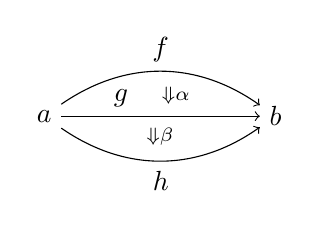
\begin{tikzpicture}[x=1.9em,y=1.35em]
      \node (a) at (0,0) {$a$};
      \node (b) at (4.4,0) {$b$};
      \draw[->] (a) to[bend left=35] node[above]{$f$} (b);
      \draw[->] (a) -- node[above,pos=0.3]{$g$} (b);
      \draw[->] (a) to[bend right=35] node[below]{$h$} (b);
      \node at (2.5,0.55) {$\scriptstyle\Downarrow\alpha$};
      \node at (2.2,-0.55) {$\scriptstyle\Downarrow\beta$};
    \end{tikzpicture}
    $\;=:\;$
    \hTwoCell{a}{b}{f}{\Downarrow\beta\cdot\alpha}{h}
    \end{center}
  \item 每支 1-\trCell{} $f\colon a\to b$ 都拥有一个恒等 2-\trCell{}
    \hTwoCell{a}{b}{f}{\Downarrow\mathrm{id}_f}{f}。
  \end{itemize}
\item 诸对象与诸 1-\trCell{}按通常的意义定义一个\trCategory；特别地，每个
  对象都拥有恒等箭头 $\mathrm{id}_{a}\colon a\to a$。
\item 诸对象与诸 2-\trCell{}构成一个\trCategory。特别地：
  \begin{itemize}
  \item 如下左图的一对 2-\trCell{}容有一个\textbf{水平复合}（horizontal
    composite），如下右图所示：
    \begin{center}
    \hTwoCell{a}{b}{f}{\Downarrow\alpha}{g}
    \hTwoCell{b}{c}{j}{\Downarrow\gamma}{k}
    $\;=:\;$
    \hTwoCell{a}{c}{jf}{\Downarrow\gamma\ast\alpha}{kg}
    \end{center}
  \item 恒等 1-\trCell{}上的恒等 2-\trCell{}
    \hTwoCell{a}{a}{\mathrm{id}_a}{\Downarrow\mathrm{id}_{\mathrm{id}_a}}{\mathrm{id}_a}
    定义水平复合的单位。
  \end{itemize}
\item 最后，水平复合相对竖直复合是函子式的：
  \begin{itemize}
  \item 恒等 2-\trCell{}的水平复合物是恒等 2-\trCell{}：
    \begin{center}
    \hTwoCell{a}{b}{g}{\Downarrow\mathrm{id}_g}{g}
    \hTwoCell{b}{c}{k}{\Downarrow\mathrm{id}_k}{k}
    $\;=\;$%
    \hTwoCell{a}{c}{kg}{\Downarrow\mathrm{id}_{kg}}{kg}
    \end{center}
  \item 在下述情形中，诸竖直复合物的水平复合与诸水平复合物的竖直复合相
    重合，这一性质被称为\textbf{中四交换}（middle-four interchange）：
    \begin{center}
    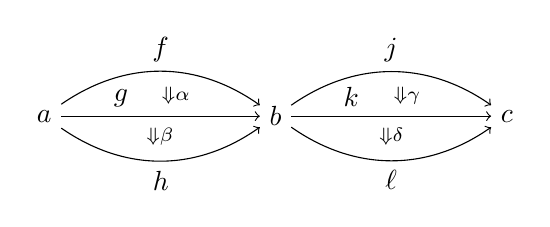
\begin{tikzpicture}[x=1.9em,y=1.35em]
      \node (a) at (0,0) {$a$};
      \node (b) at (4.4,0) {$b$};
      \node (c) at (8.8,0) {$c$};
      \draw[->] (a) to[bend left=35] node[above]{$f$} (b);
      \draw[->] (a) -- node[above,pos=0.3]{$g$} (b);
      \draw[->] (a) to[bend right=35] node[below]{$h$} (b);
      \node at (2.5,0.55) {$\scriptstyle\Downarrow\alpha$};
      \node at (2.2,-0.55) {$\scriptstyle\Downarrow\beta$};
      \draw[->] (b) to[bend left=35] node[above]{$j$} (c);
      \draw[->] (b) -- node[above,pos=0.3]{$k$} (c);
      \draw[->] (b) to[bend right=35] node[below]{$\ell$} (c);
      \node at (6.9,0.55) {$\scriptstyle\Downarrow\gamma$};
      \node at (6.6,-0.55) {$\scriptstyle\Downarrow\delta$};
    \end{tikzpicture}
    \quad
    $(\delta\ast\beta)\cdot(\gamma\ast\alpha)=(\delta\cdot\gamma)\ast(\beta\cdot\alpha)$
    \end{center}
  \end{itemize}
\end{enumerate}
\end{definition}

水平复合的一个退化特例——其中除一个 2-\trCell{}之外，其余的 2-\trCell{}都是
其边缘 1-\trCell{} $f$ 上的恒等 $\mathrm{id}_{f}$——被称为「\trWhiskering」。

\begin{definition}[\trWhiskering]\label{def:whiskering}
一个 2-\trCell{} \hTwoCell{a}{b}{f}{\Downarrow\alpha}{g} 与一对 1-\trCell{}
$k\colon x\to a$ 及 $h\colon b\to y$ 的\textbf{须状复合}（whiskered
composite）$h\alpha k$ 定义为水平复合：
\begin{center}
\hTwoCell{x}{y}{hfk}{\Downarrow h\alpha k}{hgk}
$\;:=\;$
\begin{tikzpicture}[x=1.9em,y=1.35em]
  \node (x) at (0,0) {$x$};
  \node (a) at (2.8,0) {$a$};
  \node (b) at (6.4,0) {$b$};
  \node (y) at (9.4,0) {$y$};
  \draw[->] (x) -- node[above]{$k$} (a);
  \draw[->] (a) to[bend left=30] node[above]{$f$} (b);
  \draw[->] (a) to[bend right=30] node[below]{$g$} (b);
  \node at (4.6,0) {$\scriptstyle\Downarrow\alpha$};
  \draw[->] (b) -- node[above]{$h$} (y);
\end{tikzpicture}
\\[0.5em]
$\;:=\;$
\hTwoCell{x}{a}{k}{\Downarrow\mathrm{id}_k}{k}
\hTwoCell{a}{b}{f}{\Downarrow\alpha}{g}
\hTwoCell{b}{y}{h}{\Downarrow\mathrm{id}_h}{h}
\end{center}
\end{definition}

正如下面的引理所揭示的，水平复合可以从竖直复合与\trWhiskering{}中恢复出来。
然而，我们对这一结果的主要兴趣却在于作为陈述最后一部分出现的一个相当平淡的
推论——它出人意料地经常恰其所用。

\begin{lemma}[\trWhiskering{}的自然性]\label{lem:naturality-of-whiskering}
对 2-\trCategory{}中任何可水平复合的 2-\trCell{}对，在从其定义域对象到余
定义域对象的 hom-\trCategory{}中，存在一个由诸须状胞腔组成的交换方块，其对
角线定义水平复合：
\begin{center}
$\mathcal{C}\ni$
\hTwoCell{a}{b}{f}{\Downarrow\alpha}{g}
\hTwoCell{b}{c}{h}{\Downarrow\beta}{k}
$\;\rightsquigarrow\;$
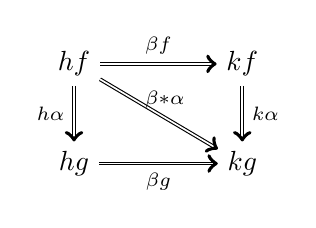
\begin{tikzpicture}[x=1.9em,y=1.5em]
  \node (hf) at (0,1.2) {$hf$};
  \node (kf) at (3.2,1.2) {$kf$};
  \node (hg) at (0,-1.2) {$hg$};
  \node (kg) at (3.2,-1.2) {$kg$};
  \draw[double,->] (hf) -- node[above]{$\scriptstyle\beta f$} (kf);
  \draw[double,->] (hf) -- node[left]{$\scriptstyle h\alpha$} (hg);
  \draw[double,->] (kf) -- node[right]{$\scriptstyle k\alpha$} (kg);
  \draw[double,->] (hg) -- node[below]{$\scriptstyle\beta g$} (kg);
  \draw[double,->] (hf) -- node[above,pos=0.55]{$\scriptstyle\beta\ast\alpha$} (kg);
\end{tikzpicture}
$\;\in\mathcal{C}(a,c)$
\end{center}
特别地，四枚须状 2-\trCell{} $h\alpha$、$k\alpha$、$\beta f$ 与 $\beta g$
中若有任何三枚可逆，则第四枚亦可逆。
\end{lemma}

\begin{proof}
由中四交换：
\begin{align*}
\beta g\cdot h\alpha
  &= (\beta\ast\mathrm{id}_g)\cdot(\mathrm{id}_h\ast\alpha)
   = (\beta\cdot\mathrm{id}_h)\ast(\mathrm{id}_g\cdot\alpha)
   = \beta\ast\alpha\\
  &= (\mathrm{id}_k\cdot\beta)\ast(\alpha\cdot\mathrm{id}_f)
   = (\mathrm{id}_k\ast\alpha)\cdot(\beta\ast\mathrm{id}_f)
   = k\alpha\cdot\beta f.
\end{align*}
\end{proof}

水平复合与竖直复合这两种操作，都是经\emph{粘贴}（pasting）而复合的特例，
后者由 Bénabou 首先引入 \cite{bib9}。其主要结果——在 2-范畴论语境中由
Power 证明 \cite{bib91}——是说，一张如下方这样良构的\trPastingDiagram{}拥有
唯一的 2-\trCell{}复合物：\footnote{此结果由\trVerity{}推广到弱 2-范畴论
语境 \cite{bib130}，在后一情形下，一旦指明其源 1-\trCell{}与靶 1-\trCell，
复合 2-\trCell{}便是良定义的（另见 \cite{bib58}）。}

\begin{rveq}\label{eq:pasting-diagram}
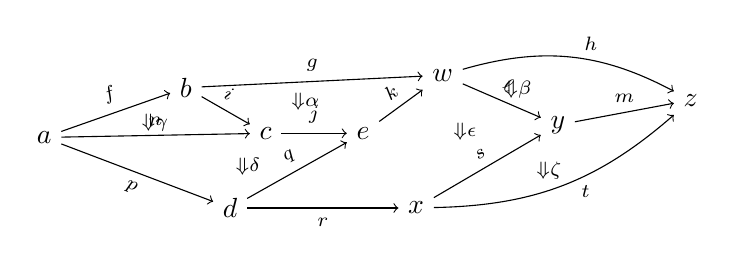
\begin{tikzpicture}[x=1.6em,y=1.5em]
  \node (a) at (0,0)      {$a$};
  \node (b) at (3.2,1.2)  {$b$};
  \node (w) at (9.0,1.5)  {$w$};
  \node (c) at (5.0,0.1)  {$c$};
  \node (e) at (7.2,0.1)  {$e$};
  \node (y) at (11.6,0.3) {$y$};
  \node (z) at (14.6,0.9) {$z$};
  \node (d) at (4.2,-1.7) {$d$};
  \node (x) at (8.4,-1.7) {$x$};
  \draw[->] (a) -- node[above,sloped]{$\scriptstyle f$} (b);
  \draw[->] (b) -- node[above]{$\scriptstyle g$} (w);
  \draw[->] (w) to[bend left=22] node[above,pos=0.6]{$\scriptstyle h$} (z);
  \draw[->] (b) -- node[above,sloped,pos=0.4]{$\scriptstyle i$} (c);
  \draw[->] (c) -- node[above]{$\scriptstyle j$} (e);
  \draw[->] (e) -- node[above,sloped]{$\scriptstyle k$} (w);
  \draw[->] (w) -- node[above,sloped]{$\scriptstyle\ell$} (y);
  \draw[->] (y) -- node[above]{$\scriptstyle m$} (z);
  \draw[->] (a) -- node[above]{$\scriptstyle n$} (c);
  \draw[->] (a) -- node[below,sloped]{$\scriptstyle p$} (d);
  \draw[->] (d) -- node[above,sloped]{$\scriptstyle q$} (e);
  \draw[->] (d) -- node[below]{$\scriptstyle r$} (x);
  \draw[->] (x) -- node[above,sloped]{$\scriptstyle s$} (y);
  \draw[->] (x) to[bend right=20] node[below,pos=0.6]{$\scriptstyle t$} (z);
  \node at (2.5,0.35)  {$\scriptstyle\Downarrow\gamma$};
  \node at (5.9,0.85)  {$\scriptstyle\Downarrow\alpha$};
  \node at (4.6,-0.7)  {$\scriptstyle\Downarrow\delta$};
  \node at (9.5,0.15)  {$\scriptstyle\Downarrow\epsilon$};
  \node at (10.7,1.15) {$\scriptstyle\Downarrow\beta$};
  \node at (11.4,-0.8) {$\scriptstyle\Downarrow\zeta$};
\end{tikzpicture}
\end{rveq}

我们将这一结果的形式陈述与证明留给文献，转而非正式地描述这类粘贴复合物应当
如何解读。

\begin{digression}[如何读取一张\trPastingDiagram]\label{dig:how-to-read-a-pasting-diagram}
2-\trCategory{} $\mathcal{C}$ 中的一张\trPastingDiagram{}表示一个唯一的复合
2-\trCell，它在对象对之间的某个 hom-\trCategory{}中定义一个态射。为了辨认
这些对象，考察\trPastingDiagram{}中对象与 1-\trCell{}的底有向图。若该%
\trPastingDiagram{}是良构的，这个图将拥有唯一的源对象 $a$ 与唯一的靶对象
$z$。这表明\trPastingDiagram{}在 hom-\trCategory{} $\mathcal{C}(a,z)$ 中
定义一个 2-\trCell。对象 $a$ 是它的\textbf{源 0-\trCell}（source 0-cell），
对象 $z$ 是它的\textbf{靶 0-\trCell}（target 0-cell）。

下一步是辨认\trPastingDiagram{}的\textbf{源 1-\trCell}（source 1-cell）与
\textbf{靶 1-\trCell}（target 1-cell）。二者都将是 $\mathcal{C}(a,z)$ 的
对象，即 2-\trCategory{}中从 $a$ 到 $z$ 的 1-\trCell。同样，若%
\trPastingDiagram{}是良构的，源 1-\trCell{}将是唯一的、由 1-\trCell{}组成的
可复合路径，其中没有任何一支作为\trPastingDiagram{}中任何 2-\trCell{}的余
定义域的一部分出现。在 \eqref{eq:pasting-diagram} 中，这些是标签出现在箭头
上方的那些 1-\trCell，其复合为 $hgf$。对偶地，靶 1-\trCell{}将是唯一的、由
1-\trCell{}组成的可复合路径，其中没有任何一支作为\trPastingDiagram{}中任何
2-\trCell{}的定义域的一部分出现。在 \eqref{eq:pasting-diagram} 中，这些是
标签出现在图表下方的那些 1-\trCell，其复合为 $trp$。

最后一步是把\trPastingDiagram{}表示为一个从 $a$ 到 $z$ 的 2-\trCell{}竖直
复合，其中每个 2-\trCell{}都是所示「原子」2-\trCell{}之一的须状复合。诸须状
原子 2-\trCell{}的源与靶描出从 $a$ 到 $z$、穿过\trPastingDiagram{}底有向图
的可复合路径，这些路径彼此仅相差「把原子 2-\trCell{}的源替换为它的靶」这一
步。\trPastingDiagram{}中的每个 2-\trCell{}都将恰好标记该复合的诸
2-\trCell{}中的一个。这些竖直 2-\trCell{}复合的表达式未必唯一，也未必穿过
每条可能的 1-\trCell{}可复合路径，不过总存在某个 2-\trCell{}的竖直复合穿过
每条 1-\trCell{}路径。

首先，在\trPastingDiagram{}中任选一个 2-\trCell，其 1-\trCell{}源可以在源
1-\trCell{}中作为一个子序列被找到；在 \eqref{eq:pasting-diagram} 中，
$\alpha$ 或 $\beta$ 皆可选作第一个。对它作\trWhiskering，使之定义一个从源
1-\trCell{} $hgf$ 到另一条从 $a$ 到 $z$、穿过该\trPastingDiagram{}的可复合
1-\trCell{}路径的 2-\trCell。于是这个须状复合便构成诸可复合 2-\trCell{}序列
的第一步。将\trPastingDiagram{}的这一部分移去并重复，直至抵达靶 1-\trCell。
在上面的例子中，共有四种可能的方式把复合粘贴胞腔 \eqref{eq:pasting-diagram}
表达为须状 2-\trCell{}的竖直复合，它们由 $\mathcal{C}(a,z)$ 中如下交换图表
的四条路径所表示：\footnote{原书此图表底行第二节点及其入边（自 $m\ell gf$ 右
行之边）的标签印作「$m\ell kjia$」与「$m\ell\alpha a$」，其末字符 $a$ 系源
0-\trCell，缀于 1-\trCell{}复合路径之末于数学不通；按顶行对应节点（$hkjif$）
与竖直边标签（$\beta kjif$）当为 $f$，此处径改。——译者注}
\begin{center}
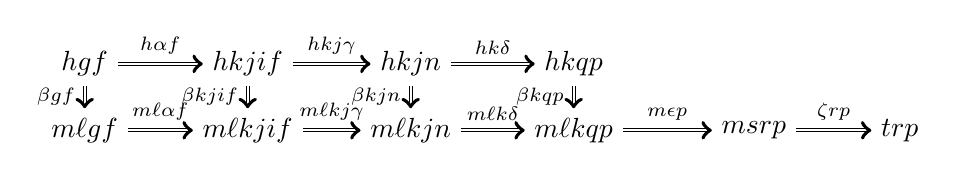
\begin{tikzpicture}[x=1.55em,y=1.6em]
  \node (t1) at (0,1.5)    {$hgf$};
  \node (t2) at (3.8,1.5)  {$hkjif$};
  \node (t3) at (7.6,1.5)  {$hkjn$};
  \node (t4) at (11.4,1.5) {$hkqp$};
  \node (b1) at (0,0)      {$m\ell gf$};
  \node (b2) at (3.8,0)    {$m\ell kjif$};
  \node (b3) at (7.6,0)    {$m\ell kjn$};
  \node (b4) at (11.4,0)   {$m\ell kqp$};
  \node (b5) at (15.6,0)   {$msrp$};
  \node (b6) at (19.0,0)   {$trp$};
  \draw[double,->] (t1) -- node[above]{$\scriptstyle h\alpha f$} (t2);
  \draw[double,->] (t2) -- node[above]{$\scriptstyle hkj\gamma$} (t3);
  \draw[double,->] (t3) -- node[above]{$\scriptstyle hk\delta$} (t4);
  \draw[double,->] (t1) -- node[left]{$\scriptstyle\beta gf$} (b1);
  \draw[double,->] (t2) -- node[left]{$\scriptstyle\beta kjif$} (b2);
  \draw[double,->] (t3) -- node[left]{$\scriptstyle\beta kjn$} (b3);
  \draw[double,->] (t4) -- node[left]{$\scriptstyle\beta kqp$} (b4);
  \draw[double,->] (b1) -- node[above]{$\scriptstyle m\ell\alpha f$} (b2);
  \draw[double,->] (b2) -- node[above]{$\scriptstyle m\ell kj\gamma$} (b3);
  \draw[double,->] (b3) -- node[above]{$\scriptstyle m\ell k\delta$} (b4);
  \draw[double,->] (b4) -- node[above]{$\scriptstyle m\epsilon p$} (b5);
  \draw[double,->] (b5) -- node[above]{$\scriptstyle\zeta rp$} (b6);
\end{tikzpicture}
\end{center}
\end{digression}

一个 2-\trCategory{}共有四个对偶（含其自身），每一者都与它拥有相同的对象、
1-\trCell{}与 2-\trCell，但会在某个维度上交换定义域与余定义域。

\begin{definition}[op-对偶与 co-对偶]\label{def:op-co-duals}
设 $\mathcal{C}$ 为一个 2-\trCategory。
\begin{itemize}
\item 它的 \textbf{op-对偶}（op-dual）$\mathcal{C}^{\mathrm{op}}$ 是满足
  $\mathcal{C}^{\mathrm{op}}(a,b):=\mathcal{C}(b,a)$ 的 2-\trCategory。它
  反转 1-\trCell{}的方向，但不反转 2-\trCell{}的方向。
\item 它的 \textbf{co-对偶}（co-dual）$\mathcal{C}^{\mathrm{co}}$ 是满足
  $\mathcal{C}^{\mathrm{co}}(a,b):=\mathcal{C}(a,b)^{\mathrm{op}}$ 的
  2-\trCategory。它反转 2-\trCell{}的方向，但不反转 1-\trCell{}的方向。
\item 它的 \textbf{coop-对偶}（coop-dual）$\mathcal{C}^{\mathrm{coop}}$ 是
  满足 $\mathcal{C}^{\mathrm{coop}}(a,b):=\mathcal{C}(b,a)^{\mathrm{op}}$
  的 2-\trCategory。它同时反转 2-\trCell{}与 1-\trCell{}的方向。
\end{itemize}
\end{definition}

我们从第 1 章中的\cref{def:equivalence-2-category}回忆起：一个 2-\trCategory{}%
中的\trEquivalence{}由下列数据给出：
\begin{itemize}
\item 一对对象 $a$ 与 $b$；
\item 一对 1-\trCell{} $f\colon a\to b$ 与 $g\colon b\to a$；
\item 一对可逆 2-\trCell\footnote{对 2-\trCell{}而言，「可逆性」的默认含义
  是对竖直复合可逆。注意，一个可逆 2-\trCell{}的边缘 1-\trCell{}未必可逆。}
  \hTwoCell{a}{a}{\mathrm{id}_a}{\cong\;\Downarrow\alpha}{gf}
  及
  \hTwoCell{b}{b}{fg}{\cong\;\Downarrow\beta}{\mathrm{id}_b}。
\end{itemize}

\begin{digression}[2-\trCategory{}内部的诸「相同」概念]\label{dig:notions-of-sameness}
从 2-范畴论的观点看，对一个 2-\trCategory{}的两个对象而言，最自然的「相同」
概念是\emph{\trEquivalence}：$a$ 与 $b$ 被视作相同的，若二者之间存在一个%
\trEquivalence。

对一个 2-\trCategory{}中一对平行的态射而言，最自然的「相同」概念是%
\emph{\trIsomorphism}：$h$，$k\colon a\to b$ 被视作相同的，若存在一个可逆
2-\trCell{} $\gamma\colon h\cong k$。

对一个具有公共边缘的 2-\trCell{}对而言，最自然的「相同」概念是\emph{相等}。由于
2-\trCategory{}缺乏任何可以在 2-\trCell{}之间作中介的更高维态射，这里没有
更弱的概念可用。
\end{digression}

在第 1 章中的\cref{dig:simplicial-categories}中，我们看到\trSimplicialCategory{}%
的数据可以表达为一个取值于 $\Cat$ 的特定类型的\trDiagram。一个小
2-\trCategory{}可以类似地被编码为——事实上以两种不同的方式——一个定义
\emph{内部}于诸\trCategory{}的\trCategory{}之中的\trCategory。

\begin{definition}[内范畴]\label{def:internal-category}
设 $\mathcal{E}$ 为任一带\trPullback{}的\trCategory。$\mathcal{E}$ 中的一个
\textbf{内范畴}（internal category）由如下数据给出
\begin{center}
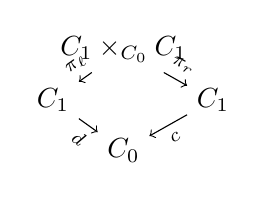
\begin{tikzpicture}[x=1.7em,y=1.3em]
  \node (t) at (1.5,2.2)  {$C_{1}\times_{C_{0}}C_{1}$};
  \node (l) at (0,0.8)    {$C_{1}$};
  \node (r) at (3.4,0.8)  {$C_{1}$};
  \node (b) at (1.5,-0.6) {$C_{0}$};
  \draw[->] (t) -- node[above,sloped]{$\scriptstyle\pi_{\ell}$} (l);
  \draw[->] (t) -- node[above,sloped]{$\scriptstyle\pi_{r}$} (r);
  \draw[->] (l) -- node[below,sloped]{$\scriptstyle d$} (b);
  \draw[->] (r) -- node[below,sloped]{$\scriptstyle c$} (b);
\end{tikzpicture}
\qquad
\rvIntCat{C_{1}\times_{C_{0}}C_{1}}{C_{1}}{C_{0}}
\end{center}
并服从一些交换图表，这些图表定义复合与单位的定义域和余定义域
\begin{center}
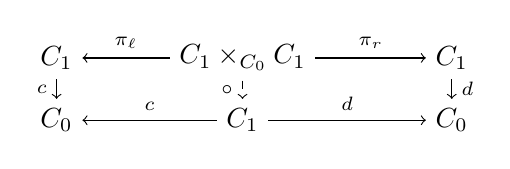
\begin{tikzpicture}[x=2.1em,y=1.5em]
  \node (tl) at (0,1.5)    {$C_{1}$};
  \node (tm) at (3.2,1.5)  {$C_{1}\times_{C_{0}}C_{1}$};
  \node (tr) at (6.8,1.5)  {$C_{1}$};
  \node (bl) at (0,0)      {$C_{0}$};
  \node (bm) at (3.2,0)    {$C_{1}$};
  \node (br) at (6.8,0)    {$C_{0}$};
  \draw[->] (tm) -- node[above]{$\scriptstyle\pi_{\ell}$} (tl);
  \draw[->] (tm) -- node[above]{$\scriptstyle\pi_{r}$} (tr);
  \draw[->] (tl) -- node[left]{$\scriptstyle c$} (bl);
  \draw[->,dashed] (tm) -- node[left]{$\scriptstyle\circ$} (bm);
  \draw[->] (tr) -- node[right]{$\scriptstyle d$} (br);
  \draw[->] (bm) -- node[above]{$\scriptstyle c$} (bl);
  \draw[->] (bm) -- node[above]{$\scriptstyle d$} (br);
\end{tikzpicture}
\qquad
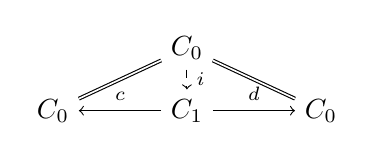
\begin{tikzpicture}[x=2.2em,y=1.5em]
  \node (t)  at (2.2,1.5) {$C_{0}$};
  \node (bl) at (0,0)     {$C_{0}$};
  \node (bm) at (2.2,0)   {$C_{1}$};
  \node (br) at (4.4,0)   {$C_{0}$};
  \draw[double] (t) -- (bl);
  \draw[double] (t) -- (br);
  \draw[->,dashed] (t) -- node[right]{$\scriptstyle i$} (bm);
  \draw[->] (bm) -- node[above]{$\scriptstyle c$} (bl);
  \draw[->] (bm) -- node[above]{$\scriptstyle d$} (br);
\end{tikzpicture}
\end{center}
并编码复合为结合且幺一这一事实。
\begin{center}
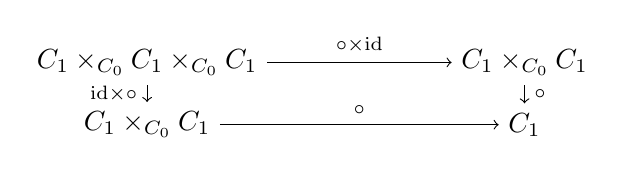
\begin{tikzpicture}[x=2.2em,y=1.5em]
  \node (tl) at (0,1.5)   {$C_{1}\times_{C_{0}}C_{1}\times_{C_{0}}C_{1}$};
  \node (tr) at (6.2,1.5) {$C_{1}\times_{C_{0}}C_{1}$};
  \node (bl) at (0,0)     {$C_{1}\times_{C_{0}}C_{1}$};
  \node (br) at (6.2,0)   {$C_{1}$};
  \draw[->] (tl) -- node[above]{$\scriptstyle\circ\times\mathrm{id}$} (tr);
  \draw[->] (tl) -- node[left]{$\scriptstyle\mathrm{id}\times\circ$} (bl);
  \draw[->] (tr) -- node[right]{$\scriptstyle\circ$} (br);
  \draw[->] (bl) -- node[above]{$\scriptstyle\circ$} (br);
\end{tikzpicture}
\qquad
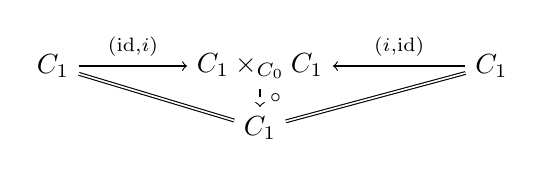
\begin{tikzpicture}[x=2.2em,y=1.5em]
  \node (l) at (0,1.5)    {$C_{1}$};
  \node (t) at (3.4,1.5)  {$C_{1}\times_{C_{0}}C_{1}$};
  \node (r) at (7.2,1.5)  {$C_{1}$};
  \node (b) at (3.4,0)    {$C_{1}$};
  \draw[->] (l) -- node[above]{$\scriptstyle(\mathrm{id},i)$} (t);
  \draw[->] (r) -- node[above]{$\scriptstyle(i,\mathrm{id})$} (t);
  \draw[->,dashed] (t) -- node[right]{$\scriptstyle\circ$} (b);
  \draw[double] (l) -- (b);
  \draw[double] (r) -- (b);
\end{tikzpicture}
\end{center}
\end{definition}

$\mathcal{S}et$ 中的一个内范畴是一个通常的小\trCategory。$\Cat$ 中的一个
内范畴定义一个\trDoubleCategory：

\begin{definition}[\trDoubleCategory]\label{def:double-category}
一个 \textbf{\trDoubleCategory} $\mathcal{C}$ 是 $\Cat$ 中的一个内范畴
\begin{center}
\rvIntCat{C_{h,s}\times_{C_{o,v}}C_{h,s}}{C_{h,s}}{C_{o,v}}
\end{center}
显式地，它拥有：
\begin{itemize}
\item 一个由对象与\textbf{竖直箭头}（vertical arrows）组成的\trCategory{}
  $C_{o,v}$；
\item 一个由\textbf{水平箭头}（horizontal arrows）与\textbf{方块}
  （squares）组成的\trCategory{} $C_{h,s}$；
\item \trFunctor{} $c$，$d\colon C_{h,s}\to C_{o,v}$，为每支水平箭头指派一
  个余定义域／定义域对象，并为每个方块指派一支余定义域／定义域竖直箭头；
\item \trFunctor{} $i\colon C_{o,v}\to C_{h,s}$，为每个对象指派一支水平恒等
  箭头，并为每支竖直箭头指派一个恒等方块；并且
\item 复合\trFunctor{} $\circ\colon C_{h,s}\times_{C_{o,v}}C_{h,s}\to C_{h,s}$，
  它定义水平箭头与方块的水平复合，且对每个变元处的竖直复合是函子式的
\end{itemize}
满足由内范畴的交换图表所强加的诸公理。
\end{definition}

一个 2-\trCategory{}可以按下列两种方式实现为这一构造的特例。

\begin{digression}[作为范畴对象的 2-\trCategory]\label{dig:two-categories-as-category-objects}
一个 2-\trCategory{}可以被定义为 $\Cat$ 中的一个内范畴
\begin{center}
\rvIntCat{C_{1,2}\times_{C_{0}}C_{1,2}}{C_{1,2}}{C_{0}}
\end{center}
其中\trCategory{} $C_{0}$ 是一个集合，即该 2-\trCategory{}的对象之集。
1-\trCell{}与 2-\trCell{}作为\trCategory{} $C_{1,2}$ 的对象与箭头出现。
\trFunctor{} $d$，$c\colon C_{1,2}\to C_{0}$ 把 1-\trCell{}与 2-\trCell{}送
到各自的定义域 0-\trCell{}与余定义域 0-\trCell。\trFunctor{}
$i\colon C_{0}\to C_{1,2}$ 把每个对象送到它的恒等 1-\trCell。\trFunctor{}
$\circ\colon C_{1,2}\times_{C_{0}}C_{1,2}\to C_{1,2}$ 在对象上的作用定义
1-\trCell{}的复合，而在态射上的作用定义 2-\trCell{}上的水平复合。2-\trCell{}%
上的竖直复合就是\trCategory{} $C_{1,2}$ 内部的复合。这一映射的\trFunctor{}性
编码了中四交换。\footnote{此定义给出了定义 E.2.4 所描述的 $(\infty,1)$-%
\trCategory{}的\trSegalCategories{}模型的动机。}

对偶地，一个 2-\trCategory{}可以被定义为 $\Cat$ 中的一个内范畴
\begin{center}
\rvIntCat{C_{0,2}\times_{C_{0,1}}C_{0,2}}{C_{0,2}}{C_{0,1}}
\end{center}
其中诸\trCategory{} $C_{0,1}$ 与 $C_{0,2}$ 拥有相同的对象之集，且全部四个%
\trFunctor{}都在对象上恒等。这里，公共的对象之集定义 2-\trCategory{}的
对象，而 $C_{0,1}$ 与 $C_{0,2}$ 的箭头分别定义 1-\trCell{}与 2-\trCell。
\trFunctor{} $d$，$c\colon C_{0,2}\to C_{0,1}$ 为一个 2-\trCell{}定义其
定义域 1-\trCell{}与余定义域 1-\trCell，而\trFunctor{}
$\circ\colon C_{0,2}\times_{C_{0,1}}C_{0,2}\to C_{0,2}$ 则编码 2-\trCell{}%
的竖直复合。\trCategory{} $C_{0,2}$ 内部的复合定义 2-\trCell{}的水平复合。
这一映射的\trFunctor{}性编码了中四交换。
\end{digression}

\subsection*{练习}

\begin{exercise}\label{ex:relate-two-category-enriched-structures}
在富集之基为 $\Cat$ 的情形下，将\cref{def:two-category}中逐项列出的诸结构，同%
附录 A 中的\cref{def:enriched-category}中逐项列出的诸结构联系起来。
\end{exercise}

\begin{exercise}\label{ex:duality-involution-double-categories}
在\trDoubleCategory{}上定义一个对偶对合（duality involution），使之交换%
\cref{dig:two-categories-as-category-objects}中出现的一个 2-\trCategory{}作为%
内范畴的两种表述。
\end{exercise}

   %

\providecommand{\Cat}{\mathcal{C}at}
\providecommand{\hTwoCell}[5]{\tikz[baseline=-0.8ex]{%
  \node (rvl) at (0,0) {$#1$};
  \node (rvr) at (2.9,0) {$#2$};
  \draw[->] (rvl) to[bend left=28] node[above]{$\scriptstyle #3$} (rvr);
  \draw[->] (rvl) to[bend right=28] node[below]{$\scriptstyle #5$} (rvr);
  \node at (1.45,0) {$\scriptstyle #4$};}}

\section{2-\trCategory{}的 3-\trCategory}\label{sec:the-3-category-of-2-categories}

通常的 1-\trCategory{}构成一个由\trCategory、\trFunctor{}与%
\trNaturalTransformation{}组成的 2-\trCategory{}的对象。类似地，2-\trCategory{}%
构成一个由 2-\trCategory、2-\trFunctor、2-\trNaturalTransformation{}与\trModification{}组成
的 3-\trCategory{}的对象。在本节中，我们将简要地介绍所有这些概念。

回忆\cref{def:two-category}：一个 2-\trCategory{}是富集于 $\Cat$ 之上的一个\trCategory。
类似地，2-\trFunctor{}与 2-\trNaturalTransformation{}恰是附录 A 中的那些
$\Cat$-富集\trFunctor{}与 $\Cat$-富集\trNaturalTransformation。由附录 A 中的%
\cref{cor:vcat-two-category}，2-\trCategory、2-\trFunctor{}与
2-\trNaturalTransformation{}拼装成一个 2-\trCategory。2-\trCategory{}之间的
$3$ 维\trCell{}——即诸\trModification{}——是利用一个 2-\trCategory{}的 2-\trCell{}来定义
的，正如 1-\trCategory{}之间的 $2$ 维\trCell{}——即诸\trNaturalTransformation{}——%
是利用一个 1-\trCategory{}中的 1-\trCell{}来定义的一样。

\begin{definition}\label{def:two-functor}
介于 2-\trCategory{}之间的一个\textbf{\trTwoFunctor}
$F\colon\mathcal{C}\to\mathcal{D}$ 由如下数据给出：
\begin{itemize}
\item 对象上的一个映射 $\mathcal{C}\ni x\mapsto Fx\in\mathcal{D}$；
\item 1-\trCell{}上的一个函子式的映射
  $\mathcal{C}\ni f\colon x\to y\mapsto Ff\colon Fx\to Fy\in\mathcal{D}$，
  保持定义域与余定义域；并且
\item 2-\trCell{}上的一个映射
\begin{center}
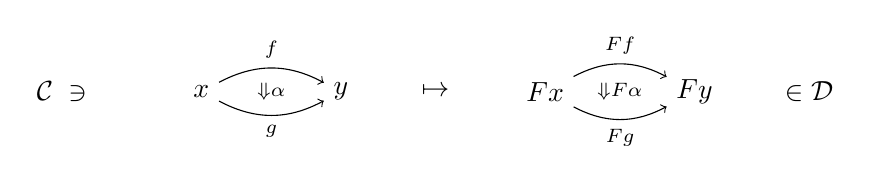
\begin{tikzpicture}[x=1.8em,y=1.5em]
  \node (C)  at (0,0)    {$\mathcal{C}\;\ni$};
  \node (x)  at (2.8,0)  {$x$};
  \node (y)  at (5.6,0)  {$y$};
  \node (mp) at (7.5,0)  {$\mapsto$};
  \node (Fx) at (9.7,0)  {$Fx$};
  \node (Fy) at (12.7,0) {$Fy$};
  \node (D)  at (15.0,0) {$\in\mathcal{D}$};
  \draw[->] (x) to[bend left=28] node[above]{$\scriptstyle f$} (y);
  \draw[->] (x) to[bend right=28] node[below]{$\scriptstyle g$} (y);
  \node at (4.2,0) {$\scriptstyle\Downarrow\alpha$};
  \draw[->] (Fx) to[bend left=28] node[above]{$\scriptstyle Ff$} (Fy);
  \draw[->] (Fx) to[bend right=28] node[below]{$\scriptstyle Fg$} (Fy);
  \node at (11.2,0) {$\scriptstyle\Downarrow F\alpha$};
\end{tikzpicture}
\end{center}
  它保持 0-\trCell{}与 1-\trCell{}的源与目标，并且对水平复合与竖直复合以及
  水平单位与竖直单位都是函子式的。
\end{itemize}
\end{definition}

\begin{definition}\label{def:two-natural-transformation}
介于一对平行 2-\trFunctor{} $F$ 与 $G$ 之间的一个%
\textbf{2-\trNaturalTransformation}（2-natural transformation）
\hTwoCell{\mathcal{C}}{\mathcal{D}}{F}{\Downarrow\phi}{G}
由 $\mathcal{D}$ 中一族 1-\trCell{}
$(\phi_{c}\colon Fc\to Gc)_{c\in\mathcal{C}}$ 给出，后者由 $\mathcal{C}$ 的诸
对象加标，且对 $\mathcal{C}$ 中的诸 1-\trCell{} $f\colon x\to y$ 自然，意即
方块
\begin{center}
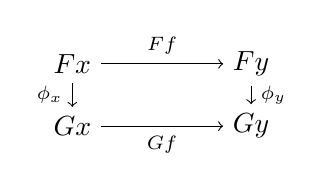
\begin{tikzpicture}[x=1.9em,y=1.5em]
  \node (tl) at (0,1.5) {$Fx$};
  \node (tr) at (3.4,1.5) {$Fy$};
  \node (bl) at (0,0) {$Gx$};
  \node (br) at (3.4,0) {$Gy$};
  \draw[->] (tl) -- node[above]{$\scriptstyle Ff$} (tr);
  \draw[->] (tl) -- node[left]{$\scriptstyle\phi_{x}$} (bl);
  \draw[->] (tr) -- node[right]{$\scriptstyle\phi_{y}$} (br);
  \draw[->] (bl) -- node[below]{$\scriptstyle Gf$} (br);
\end{tikzpicture}
\end{center}
在 $\mathcal{D}$ 中交换，并且对 $\mathcal{C}$ 中的诸 2-\trCell{}
\hTwoCell{x}{y}{f}{\Downarrow\alpha}{g}
也自然，意即诸须状复合 $\phi_{y}\cdot F\alpha$ 与
$G\alpha\cdot\phi_{x}$ 相等：
\begin{center}
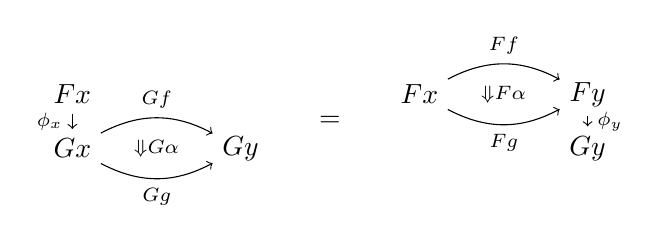
\begin{tikzpicture}[x=1.9em,y=1.5em]
  \node (LFX) at (0,1.3) {$Fx$};
  \node (LGX) at (0,0) {$Gx$};
  \node (LGY) at (3.2,0) {$Gy$};
  \draw[->] (LFX) -- node[left]{$\scriptstyle\phi_{x}$} (LGX);
  \draw[->] (LGX) to[bend left=28] node[above]{$\scriptstyle Gf$} (LGY);
  \draw[->] (LGX) to[bend right=28] node[below]{$\scriptstyle Gg$} (LGY);
  \node at (1.6,0) {$\scriptstyle\Downarrow G\alpha$};
  \node at (4.9,0.65) {$=$};
  \node (RFX) at (6.6,1.3) {$Fx$};
  \node (RFY) at (9.8,1.3) {$Fy$};
  \node (RGY) at (9.8,0) {$Gy$};
  \draw[->] (RFX) to[bend left=28] node[above]{$\scriptstyle Ff$} (RFY);
  \draw[->] (RFX) to[bend right=28] node[below]{$\scriptstyle Fg$} (RFY);
  \node at (8.2,1.3) {$\scriptstyle\Downarrow F\alpha$};
  \draw[->] (RFY) -- node[right]{$\scriptstyle\phi_{y}$} (RGY);
\end{tikzpicture}
\end{center}
\end{definition}

2-\trCategory{}之间的 $3$ 维态射居于 $\Cat$-富集\trCategory{}论的视野之外：

\begin{definition}\label{def:modification}
介于一对平行的 2-\trNaturalTransformation{}之间的一个\textbf{\trModification}
（modification）$\Xi\colon\phi\Rightarrow\psi$
\begin{center}
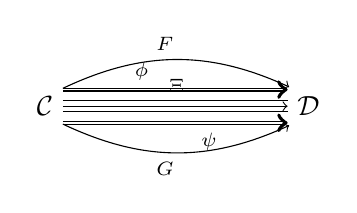
\begin{tikzpicture}[x=1.7em,y=1.5em]
  \node (C) at (0,0) {$\mathcal{C}$};
  \node (D) at (5.6,0) {$\mathcal{D}$};
  \draw[->] (C.45) to[bend left=25] node[above,pos=0.45]{$\scriptstyle F$}
    (D.135);
  \draw[->,double] ([yshift=0.6em]C.east) --
    node[above,pos=0.35]{$\scriptstyle\phi$} ([yshift=0.6em]D.west);
  \draw[->] (C.east) -- (D.west);
  \draw ([yshift=0.2em]C.east) -- ([yshift=0.2em]D.west);
  \draw ([yshift=-0.2em]C.east) -- ([yshift=-0.2em]D.west);
  \node at (2.8,0.5) {$\scriptstyle\Xi$};
  \draw[->,double] ([yshift=-0.6em]C.east) --
    node[below,pos=0.65]{$\scriptstyle\psi$} ([yshift=-0.6em]D.west);
  \draw[->] (C.-45) to[bend right=25] node[below,pos=0.45]{$\scriptstyle G$}
    (D.-135);
\end{tikzpicture}
\end{center}
由 $\mathcal{D}$ 中的如下一族 2-\trCell{}给出：
\begin{center}
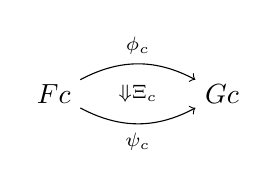
\begin{tikzpicture}[x=1.9em,y=1.5em]
  \node (a) at (0,0) {$Fc$};
  \node (b) at (3.2,0) {$Gc$};
  \draw[->] (a) to[bend left=28] node[above]{$\scriptstyle\phi_{c}$} (b);
  \draw[->] (a) to[bend right=28] node[below]{$\scriptstyle\psi_{c}$} (b);
  \node at (1.6,0) {$\scriptstyle\Downarrow\Xi_{c}$};
\end{tikzpicture}
\end{center}
其由诸对象 $c\in\mathcal{C}$ 加标，且具有如下性质：对 $\mathcal{C}$ 中的任何
1-\trCell{} $f\colon x\to y$，诸须状复合 $\Xi_{y}\cdot Ff$ 与
$Gf\cdot\Xi_{x}$ 在 $\mathcal{D}$ 中相等；并且对 $\mathcal{C}$ 中的任何
2-\trCell{} $\alpha\colon f\Rightarrow g$\footnote{原书印作「$\mathcal{D}$ 中
的任何 2-\trCell{} $\alpha\colon f\Rightarrow g$」。据下方显示式中出现的
$F\alpha$ 与 $G\alpha$，该 2-\trCell{}应居于域 2-\trCategory{} $\mathcal{C}$
之中，疑为「$\mathcal{C}$」之误，此处径改。——译者注}，诸水平复合在
$\mathcal{D}$ 中相等：
\begin{center}
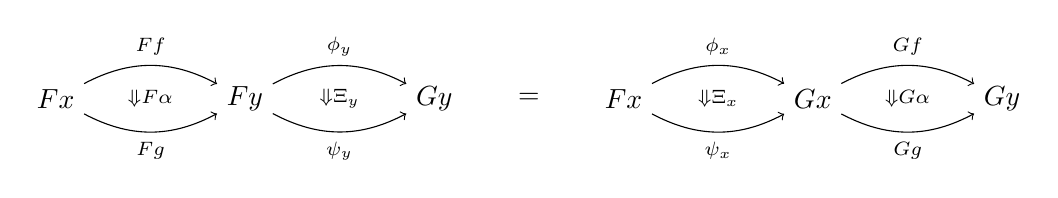
\begin{tikzpicture}[x=1.9em,y=1.5em]
  \node (Fx1) at (0,0) {$Fx$};
  \node (Fy1) at (3.6,0) {$Fy$};
  \node (Gy1) at (7.2,0) {$Gy$};
  \node (eq)  at (9.0,0) {$=$};
  \node (Fx2) at (10.8,0) {$Fx$};
  \node (Gx2) at (14.4,0) {$Gx$};
  \node (Gy2) at (18.0,0) {$Gy$};
  \draw[->] (Fx1) to[bend left=28] node[above]{$\scriptstyle Ff$} (Fy1);
  \draw[->] (Fx1) to[bend right=28] node[below]{$\scriptstyle Fg$} (Fy1);
  \node at (1.8,0) {$\scriptstyle\Downarrow F\alpha$};
  \draw[->] (Fy1) to[bend left=28] node[above]{$\scriptstyle\phi_{y}$} (Gy1);
  \draw[->] (Fy1) to[bend right=28] node[below]{$\scriptstyle\psi_{y}$} (Gy1);
  \node at (5.4,0) {$\scriptstyle\Downarrow\Xi_{y}$};
  \draw[->] (Fx2) to[bend left=28] node[above]{$\scriptstyle\phi_{x}$} (Gx2);
  \draw[->] (Fx2) to[bend right=28] node[below]{$\scriptstyle\psi_{x}$} (Gx2);
  \node at (12.6,0) {$\scriptstyle\Downarrow\Xi_{x}$};
  \draw[->] (Gx2) to[bend left=28] node[above]{$\scriptstyle Gf$} (Gy2);
  \draw[->] (Gx2) to[bend right=28] node[below]{$\scriptstyle Gg$} (Gy2);
  \node at (16.2,0) {$\scriptstyle\Downarrow G\alpha$};
\end{tikzpicture}
\end{center}
\end{definition}

由 2-\trCategory{}组成的\trCategory{}是\trCartesianClosed，其\trInternalHom{}
$\mathcal{B}^{\mathcal{A}}$ 定义为由 2-\trFunctor、2-\trNaturalTransformation{}%
与\trModification{}组成的 2-\trCategory。于是，我们现在可以把一个\textbf{3-\trCategory}定义为
富集于 2-\trCategory{}之上的一个\trCategory。

\begin{corollary}\label{cor:two-cat-three-category}
存在一个由 2-\trCategory、2-\trFunctor、2-\trNaturalTransformation{}与\trModification{}组成
的 3-\trCategory{} $2\text{-}\mathit{Cat}$。
\end{corollary}

\begin{proof}
\cref{lem:cartesian-closed-v-category}证明了：任何\trCartesianClosed{}%
\trCategory{}都富集于其自身之上。于是，$2\text{-}\mathit{Cat}$ 定义一个
3-\trCategory。
\end{proof}

\subsection*{练习}

\begin{exercise}\label{ex:relate-two-category-structures}
在富集之基为 $\Cat$ 的情形下，将\cref{def:two-functor}与%
\cref{def:two-natural-transformation}中逐项列出的诸结构，同附录 A 中的%
\cref{def:v-enriched-functor}与\cref{def:vnatural-transformation}中逐项列出的
诸结构联系起来。
\end{exercise}

\begin{exercise}\label{ex:unpack-3-category-definition}
对于拥有大块书写面的读者，请展开刚刚给出的 3-\trCategory{}的定义。
\end{exercise}

\begin{exercise}\label{ex:involutive-op-and-duals}
\begin{enumerate}[label=(\roman*)]
\item 证明：把一个 1-\trCategory{}送到其反者的那支\trFunctor{}定义一支对合
  2-\trFunctor{} $(-)^{\mathrm{op}}\colon\Cat^{\mathrm{co}}\to\Cat$，作用于由%
  \trCategory、\trFunctor{}与\trNaturalTransformation{}组成的 2-\trCategory{}%
  之上。
\item 类似地，把一个 2-\trCategory{}送到其三个对偶之一的那些\trFunctor{}可以
  被理解为由 2-\trCategory、2-\trFunctor、2-\trNaturalTransformation{}与%
  \trModification{}组成的 3-\trCategory{}的诸对合。这些映射各自具有何种变异性？
\end{enumerate}
\end{exercise}

   %

\providecommand{\Cat}{\mathcal{C}at}

\section{\trAdjunction{}与\trMate}\label{sec:adjunctions-and-mates}

正如第 2 章中所讨论的，任何 2-\trCategory{}都有一个内部定义的\trAdjunction{}概念，
由下列数据构成：
\begin{itemize}
\item 一对对象 $a$ 与 $b$；
\item 一对 1-\trCell{} $u\colon a\to b$ 与 $f\colon b\to a$；以及
\item 一对 2-\trCell{} $\eta\colon 1_{b}\Rightarrow uf$ 与
  $\epsilon\colon fu\Rightarrow 1_{a}$，分别称为\textbf{\trUnit}与%
\textbf{\trCounit}，
\end{itemize}
使得\trTriangleEqualities{}成立：
\begin{center}
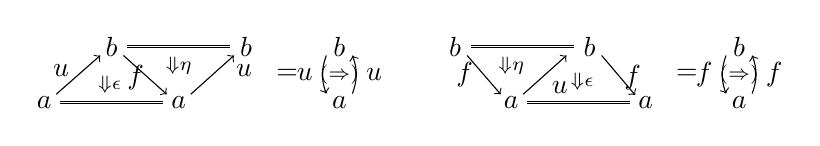
\begin{tikzpicture}[x=1.35em,y=1.35em]
  \node (A1) at (0,0) {$a$};
  \node (A2) at (3.6,0) {$a$};
  \node (B1) at (1.8,1.5) {$b$};
  \node (B2) at (5.4,1.5) {$b$};
  \draw[double] (0.42,0) -- (3.18,0);
  \draw[double] (2.22,1.5) -- (4.98,1.5);
  \draw[->] (0.32,0.22) -- (1.5,1.26);
  \node at (0.45,0.85) {$u$};
  \draw[->] (2.12,1.26) -- (3.28,0.22);
  \node at (2.45,0.68) {$f$};
  \draw[->] (3.92,0.22) -- (5.08,1.26);
  \node at (5.35,0.85) {$u$};
  \node at (1.75,0.48) {$\scriptstyle\Downarrow\epsilon$};
  \node at (3.6,1.0) {$\scriptstyle\Downarrow\eta$};
  \node at (6.5,0.75) {$=$};
  \node (Bs) at (7.9,1.5) {$b$};
  \node (As) at (7.9,0) {$a$};
  \draw[->] (7.55,1.26) to[bend right=20] node[left]{$u$} (7.55,0.24);
  \draw[->] (8.25,0.24) to[bend right=20] node[right]{$u$} (8.25,1.26);
  \node at (7.9,0.75) {$\scriptstyle(\Rightarrow)$};
  \node (B3) at (11.0,1.5) {$b$};
  \node (B4) at (14.6,1.5) {$b$};
  \node (A3) at (12.5,0) {$a$};
  \node (A4) at (16.1,0) {$a$};
  \draw[double] (11.42,1.5) -- (14.18,1.5);
  \draw[double] (12.92,0) -- (15.68,0);
  \draw[->] (11.32,1.26) -- (12.22,0.22);
  \node at (11.25,0.75) {$f$};
  \draw[->] (12.82,0.22) -- (13.98,1.26);
  \node at (13.8,0.4) {$u$};
  \draw[->] (14.92,1.26) -- (15.82,0.2);
  \node at (15.75,0.68) {$f$};
  \node at (12.5,1.0) {$\scriptstyle\Downarrow\eta$};
  \node at (14.4,0.55) {$\scriptstyle\Downarrow\epsilon$};
  \node at (17.2,0.75) {$=$};
  \node (Bt) at (18.6,1.5) {$b$};
  \node (At) at (18.6,0) {$a$};
  \draw[->] (18.25,1.26) to[bend right=20] node[left]{$f$} (18.25,0.24);
  \draw[->] (18.95,0.24) to[bend right=20] node[right]{$f$} (18.95,1.26);
  \node at (18.6,0.75) {$\scriptstyle(\Rightarrow)$};
\end{tikzpicture}
\end{center}

1-\trCell{} $f$ 称为\textbf{\trLeftAdjoint}，$u$ 称为\textbf{\trRightAdjoint}；
这一关系在行文中以 $f\dashv u$ 记之，在展示图中则画成如下之图：
\begin{rveq}\label{eq:adjunction-diagram}
\mbox{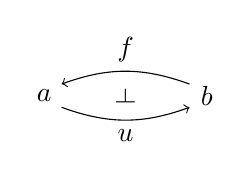
\begin{tikzpicture}[x=1.4em,y=1.4em]
  \node (a) at (0,0) {$a$};
  \node (b) at (4.2,0) {$b$};
  \draw[->] (3.75,0.3) to[bend right=20] node[above]{$f$} (0.45,0.3);
  \node[rotate=-90] at (2.1,0) {$\dashv$};
  \draw[->] (0.45,-0.3) to[bend right=20] node[below]{$u$} (3.75,-0.3);
\end{tikzpicture}}
\end{rveq}

关于\trAdjunction{}的基础 2-\trCategory{}论在 §2.1 中得到发展，其诸结果经
特殊化便可证明关于\trInfinityCategory{}之间\trAdjunction{}的定理。在此，我们沿一个
互补的方向拓广该理论——发展\emph{\trMate}（mates）的演算，它推广了人们更为熟悉的%
\trAdjunction{}转置。

当出现如 \eqref{eq:adjunction-diagram} 所示的\trAdjunction{}时，某些以 $a$ 为
余定义域的 2-\trCell{}可「转置」为以 $b$ 为余定义域的 2-\trCell{}；反对偶地，
某些以 $a$ 为定义域的 2-\trCell{}可「转置」为以 $b$ 为定义域的 2-\trCell{}：
对任何 1-\trCell{} $w\xrightarrow{x}b$、$w\xrightarrow{y}a$、$b\xrightarrow{h}z$
与 $a\xrightarrow{k}z$，
\begin{rveq}\label{eq:transposes}
fx\;\overset{\alpha}{\Longrightarrow}\;y\;\;\rightsquigarrow\;\;
x\;\overset{\beta}{\Longrightarrow}\;uy
\qquad\qquad
hu\;\overset{\gamma}{\Longrightarrow}\;k\;\;\rightsquigarrow\;\;
h\;\overset{\delta}{\Longrightarrow}\;kf
\end{rveq}
这两种转置操作都容许一个归于 Kelly 与 Street \cite{bib70} 的共同推广，称为
「\trMate」（mates correspondence），它描述由一对\trAdjunction{}所诱导的诸%
2-\trCell{}之间的一种对偶性。

\begin{definition}[\trMate]\label{def:mates}
给定任意一对\trAdjunction{}与\trFunctor
\begin{center}
\begin{tikzpicture}[x=1.9em,y=1.5em]
  \node (b)  at (0,1.5)  {$b$};
  \node (bp) at (3.6,1.5) {$b'$};
  \node (a)  at (0,0)    {$a$};
  \node (ap) at (3.6,0)  {$a'$};
  \draw[->] (0.5,1.5) -- node[above]{$\scriptstyle k$} (3.1,1.5);
  \draw[->] (0.5,0)   -- node[below]{$\scriptstyle h$} (3.1,0);
  \node[left] at (-0.25,0.75) {$f\dashv u$};
  \node[right] at (3.85,0.75) {$f'\dashv u'$};
\end{tikzpicture}
\end{center}
则在如下左侧的 2-\trCell{}与如下右侧的 2-\trCell{}之间存在一个双射
\begin{rveq}\label{eq:mates-bijection}
\mbox{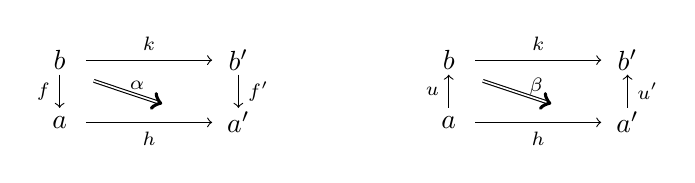
\begin{tikzpicture}[x=1.9em,y=1.5em]
  \node (lb)  at (0,1.5)  {$b$};
  \node (lbp) at (3.4,1.5) {$b'$};
  \node (la)  at (0,0)    {$a$};
  \node (lap) at (3.4,0)  {$a'$};
  \draw[->] (0.5,1.5) -- node[above]{$\scriptstyle k$} (2.9,1.5);
  \draw[->] (0.5,0)   -- node[below]{$\scriptstyle h$} (2.9,0);
  \draw[->] (0,1.15)  -- node[left]{$\scriptstyle f$} (0,0.35);
  \draw[->] (3.4,1.15) -- node[right]{$\scriptstyle f'$} (3.4,0.35);
  \draw[->,double] (0.65,1.0) -- (1.95,0.45);
  \node[right] at (1.15,0.9) {$\scriptstyle\alpha$};
  \node at (5.4,0.75) {$\rightsquigarrow$};
  \node (rb)  at (7.4,1.5)  {$b$};
  \node (rbp) at (10.8,1.5) {$b'$};
  \node (ra)  at (7.4,0)    {$a$};
  \node (rap) at (10.8,0)   {$a'$};
  \draw[->] (7.9,1.5) -- node[above]{$\scriptstyle k$} (10.3,1.5);
  \draw[->] (7.9,0)   -- node[below]{$\scriptstyle h$} (10.3,0);
  \draw[->] (7.4,0.35)  -- node[left]{$\scriptstyle u$} (7.4,1.15);
  \draw[->] (10.8,0.35) -- node[right]{$\scriptstyle u'$} (10.8,1.15);
  \draw[->,double] (8.05,1.0) -- (9.35,0.45);
  \node[right] at (8.75,0.85) {$\scriptstyle\beta$};
\end{tikzpicture}}
\end{rveq}
其通过将诸\trAdjunction{}的\trUnit{}与\trCounit{}作粘贴而实现：
\begin{center}
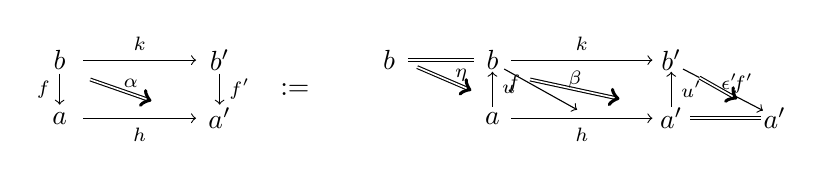
\begin{tikzpicture}[x=1.7em,y=1.4em]
  \node (ab)  at (0,1.5)  {$b$};
  \node (abp) at (3.4,1.5) {$b'$};
  \node (aa)  at (0,0)    {$a$};
  \node (aap) at (3.4,0)  {$a'$};
  \draw[->] (0.5,1.5) -- node[above]{$\scriptstyle k$} (2.9,1.5);
  \draw[->] (0.5,0)   -- node[below]{$\scriptstyle h$} (2.9,0);
  \draw[->] (0,1.15)  -- node[left]{$\scriptstyle f$} (0,0.35);
  \draw[->] (3.4,1.15) -- node[right]{$\scriptstyle f'$} (3.4,0.35);
  \draw[->,double] (0.65,1.0) -- (1.95,0.45);
  \node[right] at (1.15,0.9) {$\scriptstyle\alpha$};
  \node at (5.0,0.75) {$:=$};
  \node (pb)  at (7.0,1.5) {$b$};
  \node (pbm) at (9.2,1.5) {$b$};
  \node (pbp) at (13.0,1.5) {$b'$};
  \node (pa)  at (9.2,0) {$a$};
  \node (pam) at (13.0,0) {$a'$};
  \node (pap) at (15.2,0) {$a'$};
  \draw[double] (7.4,1.5) -- (8.8,1.5);
  \draw[->] (9.6,1.5) -- node[above]{$\scriptstyle k$} (12.6,1.5);
  \draw[->] (9.45,1.27) -- (11.0,0.22);
  \node[left] at (10.0,0.9) {$\scriptstyle f$};
  \draw[->,double] (7.6,1.32) -- (8.75,0.72);
  \node[right] at (8.2,1.1) {$\scriptstyle\eta$};
  \draw[->] (9.2,0.3) -- node[right]{$\scriptstyle u$} (9.2,1.2);
  \draw[->] (9.6,0) -- node[below]{$\scriptstyle h$} (12.6,0);
  \draw[->,double] (10.0,1.0) -- (11.9,0.5);
  \node[right] at (10.6,1.0) {$\scriptstyle\beta$};
  \draw[->] (13.0,0.3) -- node[right]{$\scriptstyle u'$} (13.0,1.2);
  \draw[->] (13.25,1.27) -- (14.95,0.2);
  \node[right] at (14.1,0.9) {$\scriptstyle f'$};
  \draw[->,double] (13.6,1.05) -- (14.4,0.5);
  \node[right] at (13.85,0.95) {$\scriptstyle\epsilon'$};
  \draw[double] (13.4,0) -- (14.9,0);
\end{tikzpicture}
\end{center}
\begin{center}
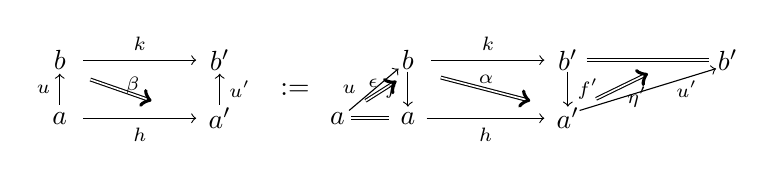
\begin{tikzpicture}[x=1.7em,y=1.4em]
  \node (bb)  at (0,1.5)  {$b$};
  \node (bbp) at (3.4,1.5) {$b'$};
  \node (ba)  at (0,0)    {$a$};
  \node (bap) at (3.4,0)  {$a'$};
  \draw[->] (0.5,1.5) -- node[above]{$\scriptstyle k$} (2.9,1.5);
  \draw[->] (0.5,0)   -- node[below]{$\scriptstyle h$} (2.9,0);
  \draw[->] (0,0.35)  -- node[left]{$\scriptstyle u$} (0,1.15);
  \draw[->] (3.4,0.35) -- node[right]{$\scriptstyle u'$} (3.4,1.15);
  \draw[->,double] (0.65,1.0) -- (1.95,0.45);
  \node[right] at (1.2,0.85) {$\scriptstyle\beta$};
  \node at (5.0,0.75) {$:=$};
  \node (qb)  at (7.4,1.5) {$b$};
  \node (qbp) at (10.8,1.5) {$b'$};
  \node (qbp2) at (14.2,1.5) {$b'$};
  \node (qa)  at (5.9,0) {$a$};
  \node (qam) at (7.4,0) {$a$};
  \node (qap) at (10.8,0) {$a'$};
  \draw[->] (7.9,1.5) -- node[above]{$\scriptstyle k$} (10.3,1.5);
  \draw[double] (11.2,1.5) -- (13.8,1.5);
  \draw[->] (6.15,0.2) -- (7.2,1.28);
  \node[left] at (6.5,0.75) {$\scriptstyle u$};
  \draw[->,double] (6.5,0.45) -- (7.15,0.95);
  \node[right] at (6.35,0.9) {$\scriptstyle\epsilon$};
  \draw[->] (7.4,1.2) -- node[left]{$\scriptstyle f$} (7.4,0.3);
  \draw[double] (6.2,0) -- (7.0,0);
  \draw[->] (7.8,0) -- node[below]{$\scriptstyle h$} (10.3,0);
  \draw[->,double] (8.1,1.05) -- (10.0,0.45);
  \node[right] at (8.7,1.0) {$\scriptstyle\alpha$};
  \draw[->] (10.8,1.2) -- node[right]{$\scriptstyle f'$} (10.8,0.3);
  \draw[->] (11.05,0.2) -- (13.95,1.28);
  \node[right] at (12.9,0.75) {$\scriptstyle u'$};
  \draw[->,double] (11.4,0.5) -- (12.5,1.15);
  \node[right] at (11.85,0.55) {$\scriptstyle\eta'$};
\end{tikzpicture}
\end{center}
\end{definition}

在该双射下相互对应的诸 2-\trCell{} \eqref{eq:mates-bijection} 称为%
\textbf{\trMate}（mates）。

\begin{example}\label{exa:conjugates}
这一\trMate{}可特殊化而定义一个双射：一边是介于一对平行的\trLeftAdjoint{}之间的%
2-\trCell，另一边是以相反方向介于它们的\trRightAdjoint{}之间的 2-\trCell——
Mac Lane 称之为\textbf{\trConjugate}（conjugates）\cite[\S IV.7]{bib81}：
\begin{center}
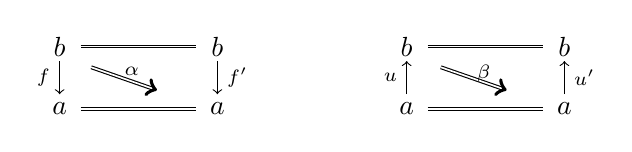
\begin{tikzpicture}[x=1.9em,y=1.5em]
  \node (cb) at (0,1.5)  {$b$};
  \node (cb2) at (3.0,1.5) {$b$};
  \node (ca) at (0,0)    {$a$};
  \node (ca2) at (3.0,0) {$a$};
  \draw[double] (0.4,1.5) -- (2.6,1.5);
  \draw[double] (0.4,0)   -- (2.6,0);
  \draw[->] (0,1.15)  -- node[left]{$\scriptstyle f$} (0,0.35);
  \draw[->] (3.0,1.15) -- node[right]{$\scriptstyle f'$} (3.0,0.35);
  \draw[->,double] (0.6,1.0) -- (1.85,0.45);
  \node[right] at (1.05,0.9) {$\scriptstyle\alpha$};
  \node at (4.8,0.75) {$\rightsquigarrow$};
  \node (db) at (6.6,1.5)  {$b$};
  \node (db2) at (9.6,1.5) {$b$};
  \node (da) at (6.6,0)    {$a$};
  \node (da2) at (9.6,0)   {$a$};
  \draw[double] (7.0,1.5) -- (9.2,1.5);
  \draw[double] (7.0,0)   -- (9.2,0);
  \draw[->] (6.6,0.35)  -- node[left]{$\scriptstyle u$} (6.6,1.15);
  \draw[->] (9.6,0.35)  -- node[right]{$\scriptstyle u'$} (9.6,1.15);
  \draw[->,double] (7.25,1.0) -- (8.5,0.45);
  \node[right] at (7.75,0.85) {$\scriptstyle\beta$};
\end{tikzpicture}
\end{center}
\end{example}

方块 \eqref{eq:mates-bijection} 的水平复合与竖直复合都保持这一\trMate，其确切
含义由如下结果阐明：

\begin{theorem}[\trMate{}的双函子性]\label{thm:mates-double-functoriality}
对任何 2-\trCategory，介于诸\trDoubleCategory{}之间存在一个双\trIsomorphism
$\mathbb{L}_{\mathrm{adj}}\cong\mathbb{R}_{\mathrm{adj}}$，这些\trDoubleCategory{}满足：
\begin{itemize}
\item 其对象与水平态射即诸对象与诸 1-\trCell；
\item 其竖直态射为完整指定的诸\trAdjunction{} $(f,u,\eta,\epsilon)$，指向%
\trLeftAdjoint{}的方向；\footnote{竖直态射的复合用到第 2 章中的%
\cref{prop:adjunctions-compose}的证明中给出的构造。}
\item $\mathbb{L}_{\mathrm{adj}}$ 中的胞腔是下方左侧所示形状的 2-\trCell，而
  $\mathbb{R}_{\mathrm{adj}}$ 中的胞腔是下方右侧所示形状的 2-\trCell：
\begin{center}
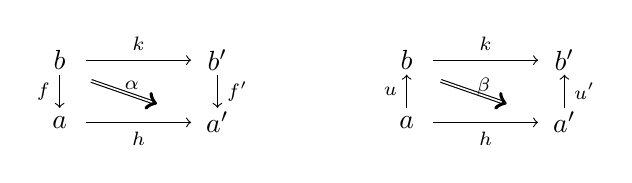
\begin{tikzpicture}[x=1.9em,y=1.5em]
  \node (eb) at (0,1.5) {$b$};
  \node (ebp) at (3.0,1.5) {$b'$};
  \node (ea) at (0,0) {$a$};
  \node (eap) at (3.0,0) {$a'$};
  \draw[->] (0.5,1.5) -- node[above]{$\scriptstyle k$} (2.5,1.5);
  \draw[->] (0.5,0)   -- node[below]{$\scriptstyle h$} (2.5,0);
  \draw[->] (0,1.15)  -- node[left]{$\scriptstyle f$} (0,0.35);
  \draw[->] (3.0,1.15) -- node[right]{$\scriptstyle f'$} (3.0,0.35);
  \draw[->,double] (0.6,1.0) -- (1.85,0.45);
  \node[right] at (1.05,0.9) {$\scriptstyle\alpha$};
  \node (fb) at (6.6,1.5) {$b$};
  \node (fbp) at (9.6,1.5) {$b'$};
  \node (fa) at (6.6,0) {$a$};
  \node (fap) at (9.6,0) {$a'$};
  \draw[->] (7.1,1.5) -- node[above]{$\scriptstyle k$} (9.1,1.5);
  \draw[->] (7.1,0)   -- node[below]{$\scriptstyle h$} (9.1,0);
  \draw[->] (6.6,0.35)  -- node[left]{$\scriptstyle u$} (6.6,1.15);
  \draw[->] (9.6,0.35)  -- node[right]{$\scriptstyle u'$} (9.6,1.15);
  \draw[->,double] (7.25,1.0) -- (8.5,0.45);
  \node[right] at (7.75,0.85) {$\scriptstyle\beta$};
\end{tikzpicture}
\end{center}
\end{itemize}
这一双\trIsomorphism{}在对象以及水平与竖直态射上充当恒等，而在胞腔上的作用
则是取\trMate。\footnote{\trDoubleCategory{}的这个双\trIsomorphism{}可视为定义了一个 2-自然%
\trIsomorphism{}的某个分量，而该 2-自然\trIsomorphism{}则介于 2-\trFunctor{}
$\mathbb{L}_{\mathrm{adj}}$、$\mathbb{R}_{\mathrm{adj}}\colon 2\text{-}\mathit{Cat}\to\mathsf{Dbl}\text{-}\mathit{Cat}$
之间——后者从 $2\text{-}\mathit{Cat}$ 映到由\trDoubleCategory、
双\trFunctor{}与水平\trNaturalTransformation{}组成的 2-\trCategory。}
\end{theorem}

\begin{proof}
这一\trMate{}的水平与竖直函子性可通过在\trPastingDiagram{}中追图来验证
（或参见 \cite[2.2]{bib70}）。
\end{proof}

\begin{warning}[同构的\trMate{}未必是同构]\label{war:mates-of-isomorphisms}
一般地说，\eqref{eq:mates-bijection} 的一对相互对应的 2-\trCell{}之中的某一个
可为\trInvertible{}而另一个不然。例如，\trAdjunction{} $f\dashv u$ 的\trUnit{}与%
\trCounit{}各自既可与恒等\trCell{} $\mathrm{id}_{f}$ 相对应、又可与恒等\trCell
$\mathrm{id}_{u}$ 相对应，视这些 2-\trCell{}以何种方式被安放进方块而定
（见\cref{ex:mates-identity-cells}）。然而，若两个水平 1-\trCell{} $h$ 与 $k$
都是\trEquivalence，或者两个\trAdjunction{} $f\dashv u$ 与 $f'\dashv u'$ 都是%
\trAdjointEquivalence，则 $\alpha\colon f'k\Rightarrow hf$ 是\trInvertible
当且仅当其\trMate{} $\beta\colon ku\Rightarrow u'h$ 是\trInvertible。
\end{warning}

在\cref{war:mates-of-isomorphisms}的基础上，我们有：

\begin{proposition}[伴随性的等价不变性]\label{prop:equivalence-invariance-of-adjointness}
设给定一个本质交换的方块，其水平箭头均为\trEquivalence：
\begin{center}
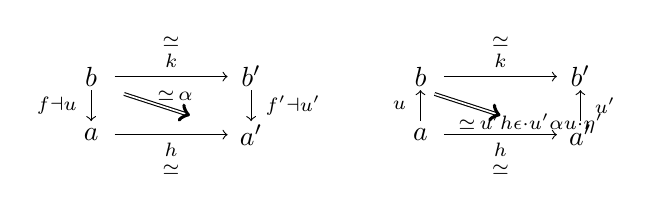
\begin{tikzpicture}[x=1.7em,y=1.4em]
  \node (gb) at (1.4,1.5) {$b$};
  \node (gbp) at (4.8,1.5) {$b'$};
  \node (ga) at (1.4,0) {$a$};
  \node (gap) at (4.8,0) {$a'$};
  \draw[->] (1.9,1.5) -- (4.3,1.5);
  \node at (3.1,1.9) {$\scriptstyle k$};
  \node at (3.1,2.4) {$\scriptstyle\simeq$};
  \draw[->] (1.9,0) -- (4.3,0);
  \node at (3.1,-0.4) {$\scriptstyle h$};
  \node at (3.1,-0.9) {$\scriptstyle\simeq$};
  \draw[->] (1.4,1.15) -- (1.4,0.35);
  \node[left] at (1.3,0.75) {$\scriptstyle f\dashv u$};
  \draw[->] (4.8,1.15) -- (4.8,0.35);
  \node[right] at (4.9,0.75) {$\scriptstyle f'\dashv u'$};
  \draw[->,double] (2.1,1.05) -- (3.5,0.5);
  \node[right] at (2.6,1.0) {$\scriptstyle\simeq\,\alpha$};
  \node at (6.6,0.75) {$\rightsquigarrow$};
  \node (hb) at (8.4,1.5) {$b$};
  \node (hbp) at (11.8,1.5) {$b'$};
  \node (ha) at (8.4,0) {$a$};
  \node (hap) at (11.8,0) {$a'$};
  \draw[->] (8.9,1.5) -- (11.3,1.5);
  \node at (10.1,1.9) {$\scriptstyle k$};
  \node at (10.1,2.4) {$\scriptstyle\simeq$};
  \draw[->] (8.9,0) -- (11.3,0);
  \node at (10.1,-0.4) {$\scriptstyle h$};
  \node at (10.1,-0.9) {$\scriptstyle\simeq$};
  \draw[->] (8.4,0.35) -- (8.4,1.15);
  \node[left] at (8.3,0.75) {$\scriptstyle u$};
  \draw[->] (11.8,0.35) -- (11.8,1.15);
  \node[right] at (11.9,0.75) {$\scriptstyle u'$};
  \draw[->,double] (8.7,1.05) -- (10.1,0.5);
  \node[right] at (9.0,0.28) {$\scriptstyle\simeq\,u'h\epsilon\cdot u'\alpha u\cdot\eta'$};
\end{tikzpicture}
\end{center}
则 $f$ 容许一个\trRightAdjoint{} $u$，当且仅当 $f'$ 容许一个\trRightAdjoint{}
$u'$；此时，同构 $\alpha$ 的\trMate{}是一个\trIsomorphism。
\end{proposition}

\begin{proof}
第 2 章中的\cref{prop:adjoint-equivalences}可用来选取互逆的\trAdjointEquivalence
$k'\dashv k$ 与 $h\dashv h'$。若 $f$ 是一个\trLeftAdjoint，则由第 2 章中的%
\cref{prop:adjunctions-compose}，$f'\cong hfk'$ 同构于一个\trLeftAdjoint，于是由
第 2 章中的\cref{prop:uniqueness-of-adjoints}，$f'$ 是 $kuh'$ 的\trLeftAdjoint。
$f'\dashv u'$ 被定义为如前一段所示的复合\trAdjunction，则 $\alpha$ 的\trMate{}算出来
是 $h'h\cong\mathrm{id}_{a}$ 与 $ku$ 的须状复合。由第 2 章中的%
\cref{prop:uniqueness-of-adjoints}，$f'$ 的\trRightAdjoint{}的任何其他选取都与
这一个同构，故 $\alpha$ 的\trMate{}仍是一个\trIsomorphism。
\end{proof}

\cref{ex:left-adjoints-isomorphic}提示了一个新证明：拥有公共右伴随的任意一对%
\trLeftAdjoint{} $f'\dashv u$ 与 $f\dashv u$ 都是同构的
（见第 2 章中的\cref{prop:uniqueness-of-adjoints}）——只需运用双%
\trIsomorphism{} $\mathbb{L}_{\mathrm{adj}}\cong\mathbb{R}_{\mathrm{adj}}$。
沿同一路线的一个更复杂的论证则可用来证明：

\begin{lemma}\label{lem:adjoint-triple-invertible-cells}
设给定\trFunctor{}的一个\trAdjointTriple{} $\ell\dashv i\dashv r$。则 $\ell\dashv i$
的\trCounit{}是\trInvertible，当且仅当 $i\dashv r$ 的\trUnit{}是\trInvertible。
\end{lemma}

\begin{proof}
设 $i\colon a\to b$，并记 $\epsilon\colon\ell i\Rightarrow\mathrm{id}_{a}$ 为
$\ell\dashv i$ 的\trCounit、$\eta\colon\mathrm{id}_{a}\Rightarrow ri$ 为
$i\dashv r$ 的\trUnit。若 $\epsilon$ 容许一个逆\trIsomorphism
$\epsilon^{-1}\colon\mathrm{id}_{a}\Rightarrow\ell i$%
\footnote{原书印作「$\epsilon^{-1}\colon\ell i\Rightarrow\mathrm{id}_{a}$」，
与 $\epsilon$ 同向。逆\trIsomorphism{}的方向应当相反，且本节下文总结处原书
亦自印作「$\epsilon^{-1}\colon\mathrm{id}_{a}\Rightarrow\ell i$」，疑为笔误，
此处径改。——译者注}，则下方左侧所示的 $\mathbb{L}_{\mathrm{adj}}$ 中的竖直
复合，容许下方右侧所示的胞腔作为其关于水平复合的逆：
\begin{center}
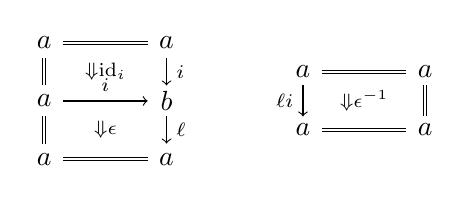
\begin{tikzpicture}[x=1.7em,y=1.4em]
  \node (m1) at (0,3) {$a$};
  \node (m2) at (2.6,3) {$a$};
  \draw[double] (0.4,3) -- (2.2,3);
  \draw[double] (0,2.6) -- (0,1.9);
  \draw[->] (2.6,2.6) -- node[right]{$\scriptstyle i$} (2.6,1.9);
  \node at (1.3,2.25) {$\scriptstyle\Downarrow\mathrm{id}_{i}$};
  \node (m3) at (0,1.5) {$a$};
  \node (m4) at (2.6,1.5) {$b$};
  \draw[->] (0.4,1.5) -- node[above]{$\scriptstyle i$} (2.2,1.5);
  \draw[double] (0,1.1) -- (0,0.4);
  \draw[->] (2.6,1.1) -- node[right]{$\scriptstyle\ell$} (2.6,0.4);
  \node at (1.3,0.75) {$\scriptstyle\Downarrow\epsilon$};
  \node (m5) at (0,0) {$a$};
  \node (m6) at (2.6,0) {$a$};
  \draw[double] (0.4,0) -- (2.2,0);
  \node (n1) at (5.5,2.25) {$a$};
  \node (n2) at (8.1,2.25) {$a$};
  \draw[double] (5.9,2.25) -- (7.7,2.25);
  \draw[->] (5.5,1.9) -- node[left]{$\scriptstyle\ell i$} (5.5,1.1);
  \draw[double] (8.1,1.9) -- (8.1,1.1);
  \node at (6.8,1.5) {$\scriptstyle\Downarrow\epsilon^{-1}$};
  \node (n3) at (5.5,0.75) {$a$};
  \node (n4) at (8.1,0.75) {$a$};
  \draw[double] (5.9,0.75) -- (7.7,0.75);
\end{tikzpicture}
\end{center}
运用双\trIsomorphism{} $\mathbb{L}_{\mathrm{adj}}\cong\mathbb{R}_{\mathrm{adj}}$
的水平函子性，这些胞腔的诸\trMate{}在 $\mathbb{R}_{\mathrm{adj}}$ 中水平复合亦必成为
恒等。\footnote{由于所论胞腔中的水平态射皆为恒等，\cref{war:mates-of-isomorphisms}中提出的顾虑在此并不适用。}运用双%
\trIsomorphism{} $\mathbb{L}_{\mathrm{adj}}\cong\mathbb{R}_{\mathrm{adj}}$ 的
竖直函子性，该竖直复合的\trMate{}等于 $\mathbb{R}_{\mathrm{adj}}$ 中的如下复合：
\begin{center}
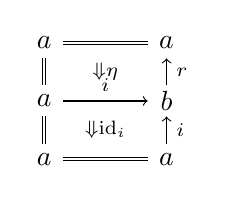
\begin{tikzpicture}[x=1.7em,y=1.4em]
  \node (o1) at (0,3) {$a$};
  \node (o2) at (2.6,3) {$a$};
  \draw[double] (0.4,3) -- (2.2,3);
  \draw[double] (0,2.6) -- (0,1.9);
  \draw[->] (2.6,1.9) -- node[right]{$\scriptstyle r$} (2.6,2.6);
  \node at (1.3,2.25) {$\scriptstyle\Downarrow\eta$};
  \node (o3) at (0,1.5) {$a$};
  \node (o4) at (2.6,1.5) {$b$};
  \draw[->] (0.4,1.5) -- node[above]{$\scriptstyle i$} (2.2,1.5);
  \draw[double] (0,1.1) -- (0,0.4);
  \draw[->] (2.6,0.4) -- node[right]{$\scriptstyle i$} (2.6,1.1);
  \node at (1.3,0.75) {$\scriptstyle\Downarrow\mathrm{id}_{i}$};
  \node (o5) at (0,0) {$a$};
  \node (o6) at (2.6,0) {$a$};
  \draw[double] (0.4,0) -- (2.2,0);
\end{tikzpicture}
\end{center}
从而 $\epsilon^{-1}$ 的\trMate{}必给出 $\eta$ 的逆。总而言之，我们看到：$\ell\dashv i$
的\trCounit{}是一个\trIsomorphism，当且仅当 $i\dashv r$ 的\trUnit{}是一个%
\trIsomorphism；此时，其逆\trIsomorphism{}
$\eta^{-1}\colon ri\Rightarrow\mathrm{id}_{a}$
便是 $\epsilon^{-1}\colon\mathrm{id}_{a}\Rightarrow\ell i$
经由复合\trAdjunction{} $\ell i\dashv ri$ 而得的\trConjugate{}：
\begin{center}
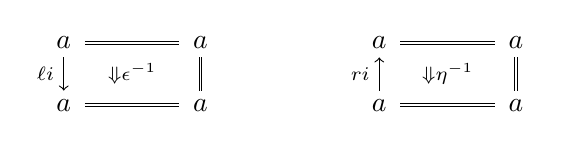
\begin{tikzpicture}[x=1.9em,y=1.5em]
  \node (p1) at (0,1.5) {$a$};
  \node (p2) at (2.6,1.5) {$a$};
  \draw[double] (0.4,1.5) -- (2.2,1.5);
  \draw[->] (0,1.15) -- node[left]{$\scriptstyle\ell i$} (0,0.35);
  \draw[double] (2.6,1.15) -- (2.6,0.35);
  \node at (1.3,0.75) {$\scriptstyle\Downarrow\epsilon^{-1}$};
  \node (p3) at (0,0) {$a$};
  \node (p4) at (2.6,0) {$a$};
  \draw[double] (0.4,0) -- (2.2,0);
  \node at (4.3,0.75) {$\rightsquigarrow$};
  \node (q1) at (6.0,1.5) {$a$};
  \node (q2) at (8.6,1.5) {$a$};
  \draw[double] (6.4,1.5) -- (8.2,1.5);
  \draw[->] (6.0,0.35) -- node[left]{$\scriptstyle ri$} (6.0,1.15);
  \draw[double] (8.6,1.15) -- (8.6,0.35);
  \node at (7.3,0.75) {$\scriptstyle\Downarrow\eta^{-1}$};
  \node (q3) at (6.0,0) {$a$};
  \node (q4) at (8.6,0) {$a$};
  \draw[double] (6.4,0) -- (8.2,0);
\end{tikzpicture}
\end{center}
\end{proof}

\subsection*{练习}

\begin{exercise}\label{ex:mates-identity-cells}
\begin{enumerate}[label=(\roman*)]
\item 说明 \eqref{eq:transposes} 的诸双射如何可以实现为\trMate{}的特殊情形。
\item 通过选取一对合适的\trAdjunction{}与\trFunctor，说明\trAdjunction{}
  $f\dashv u$ 的\trUnit{}如何与 $\mathrm{id}_{u}$ 相对应。
\item 通过选取一对合适的\trAdjunction{}与\trFunctor，说明\trAdjunction{}
  $f\dashv u$ 的\trUnit{}如何与 $\mathrm{id}_{f}$ 相对应。
\end{enumerate}
\end{exercise}

\begin{exercise}\label{ex:left-adjoints-isomorphic}
考虑 $\mathbb{L}_{\mathrm{adj}}\cong\mathbb{R}_{\mathrm{adj}}$ 中作为竖直态射的
一对\trAdjunction{} $f\dashv u$ 与 $f'\dashv u$，并运用\trMate{}的双函子性证明
$f\cong f'$。
\end{exercise}

\begin{exercise}\label{ex:horizontal-vertical-mates}
考虑 2-\trCell
\begin{center}
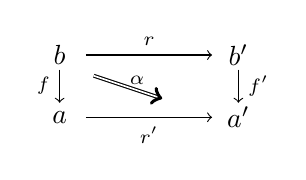
\begin{tikzpicture}[x=1.9em,y=1.5em]
  \node (wb)  at (0,1.5)  {$b$};
  \node (wbp) at (3.4,1.5) {$b'$};
  \node (wa)  at (0,0)    {$a$};
  \node (wap) at (3.4,0)  {$a'$};
  \draw[->] (0.5,1.5) -- node[above]{$\scriptstyle r$} (2.9,1.5);
  \draw[->] (0.5,0)   -- node[below]{$\scriptstyle r'$} (2.9,0);
  \draw[->] (0,1.15)  -- node[left]{$\scriptstyle f$} (0,0.35);
  \draw[->] (3.4,1.15) -- node[right]{$\scriptstyle f'$} (3.4,0.35);
  \draw[->,double] (0.65,1.0) -- (1.95,0.45);
  \node[right] at (1.15,0.9) {$\scriptstyle\alpha$};
\end{tikzpicture}
\end{center}
其中竖直 1-\trCell{}容许\trRightAdjoint{} $f\dashv u$ 与 $f'\dashv u'$，水平
1-\trCell{}容许\trLeftAdjoint{} $\ell\dashv r$ 与 $\ell'\dashv r'$。证明：$\alpha$
关于诸竖直\trAdjunction{}的\trMate{}定义一个\trIsomorphism{} $ru\cong u'r'$，当且仅当
$\alpha$ 关于诸水平\trAdjunction{}的\trMate{}定义一个\trIsomorphism{}
$\ell'f'\cong f\ell$——并且，就诸复合\trAdjunction{}而言，这两个\trIsomorphism{}%
本身即在\cref{exa:conjugates}的意义下相互对应。
\end{exercise}

\begin{exercise}\label{ex:two-functor-preserves-mates}
证明任何 2-\trFunctor{} $F\colon\mathcal{C}\to\mathcal{D}$ 都保持%
\trEquivalence、\trAdjunction{}与\trMate。
\end{exercise}

   %

\providecommand{\hTwoCell}[5]{\tikz[baseline=-0.8ex]{%
  \node (rvl) at (0,0) {$#1$};
  \node (rvr) at (2.9,0) {$#2$};
  \draw[->] (rvl) to[bend left=28] node[above]{$\scriptstyle #3$} (rvr);
  \draw[->] (rvl) to[bend right=28] node[below]{$\scriptstyle #5$} (rvr);
  \node at (1.45,0) {$\scriptstyle #4$};}}

\section{右伴随右逆伴随}\label{sec:right-adjoint-right-inverse-adjunctions}

一类重要的\trAdjunction，是其\trCounit{}可逆的那些\trAdjunction。

\begin{definition}[右伴随右逆]\label{def:rajri}
2-\trCategory{}中的一支 1-\trCell{} $f\colon b\to a$ 容许一个%
\textbf{\trRightAdjoint\trRightInverse}，若它容许一个\trRightAdjoint{} $u\colon a\to b$
使得\trAdjunction{} $f\dashv u$ 的\trCounit{}是一个\trIsomorphism。在这种情形下，$f$ 是
$u$ 的\textbf{左伴随左逆}。
\end{definition}

余对偶则定义了带可逆单位的\textbf{\trLeftAdjoint\trRightInverse}或%
\textbf{右伴随左逆}（right adjoint left inverse）伴随类。

当 $f\dashv u$ 的\trCounit{}是一个\trIsomorphism{}时，其\trUnit{}的诸须状复合
$f\eta$ 与 $\eta u$ 也必是\trIsomorphism。事实上，要构造一个这种形式的\trAdjunction，
只需给出具有这些性质的诸 2-\trCell{}即可，正如下面这条 2-范畴引理所证明的那样。

\begin{lemma}\label{lem:rajri-modification}
设在 2-\trCategory{}中给定一对 1-\trCell{} $u\colon a\to b$ 与 $f\colon b\to a$，以及一
个 2-\trIsomorphism{} $fu\cong\mathrm{id}_{a}$。若存在 2-\trCell{}
$\eta'\colon\mathrm{id}_{b}\Rightarrow uf$ 使得 $f\eta'$ 与 $\eta'u$ 都是
2-\trIsomorphism，则 $f$ 左伴随于 $u$。此外，在 $u$ 是 $f$ 的\trSection{}这一特殊情形
下，$f$ 左伴随于 $u$，且该\trAdjunction{}的\trCounit{}为恒等。
\end{lemma}

由于 $f\eta'$ 与 $\eta'u$ 都是\trIsomorphism，而 $fu\cong\mathrm{id}_{a}$，第 2 章中的%
\cref{lem:minimal-adjunction-data}的那些「三角等式复合」便是可逆的，于是由该结果即可
得出 $f\dashv u$。事实上，从该证明中给出的构造可以看到，我们可以取所指定的同构
$fu\cong\mathrm{id}_{a}$ 来作这个\trAdjunction{}的\trCounit，因此特别地，当 $u$ 是 $f$
的\trSection{}时，这个\trCounit{}便可取为恒等。下面给出的直接证明便是把刚才概述的论证
加以展开。

\begin{proof}
设 $\epsilon\colon fu\Rightarrow\mathrm{id}_{a}$ 为此同构，在 $u$ 是 $f$ 的\trSection{}%
的情形下取它为恒等。我们将通过修改 $\eta'\colon\mathrm{id}_{b}\Rightarrow uf$ 来定义一
个以 $\epsilon$ 为\trCounit{}的\trAdjunction{} $f\dashv u$。「三角等式复合」
$\theta\coloneqq u\epsilon\cdot\eta'u\colon u\Rightarrow u$ 定义了 $u$ 的一个自同构。
定义
\[
\eta \coloneqq \mathrm{id}_{b} \xRightarrow{\;\eta'\;} uf
  \xRightarrow{\;\theta^{-1}f\;} uf
\coloneqq \mathrm{id}_{b} \xRightarrow{\;\eta'\;} uf
  \xRightarrow{\;(u\epsilon f)^{-1}\;} ufuf
  \xRightarrow{\;(\eta' uf)^{-1}\;} uf.
\]
立即可得 $u\epsilon\cdot\eta u=\mathrm{id}_{u}$，这由如下计算加以验证：
\begin{center}
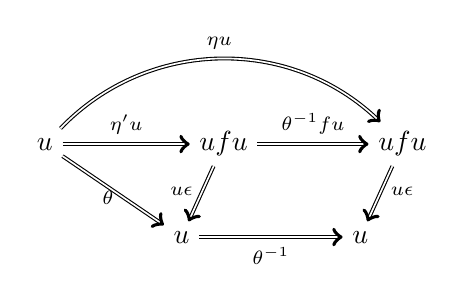
\begin{tikzpicture}[x=1.9em,y=1.4em]
  \node (u1)   at (0,1.2)    {$u$};
  \node (ufu1) at (3.4,1.2)  {$ufu$};
  \node (ufu2) at (6.8,1.2)  {$ufu$};
  \node (u2)   at (2.6,-1.2) {$u$};
  \node (u3)   at (6,-1.2)   {$u$};
  \draw[double,->] (u1) -- node[above]{$\scriptstyle\eta'u$} (ufu1);
  \draw[double,->] (ufu1) -- node[above]{$\scriptstyle\theta^{-1}fu$} (ufu2);
  \draw[double,->] (u1) to[bend left=45]
    node[above,pos=0.5]{$\scriptstyle\eta u$} (ufu2);
  \draw[double,->] (ufu1) -- node[left,pos=0.45]{$\scriptstyle u\epsilon$} (u2);
  \draw[double,->] (ufu2) -- node[right,pos=0.45]{$\scriptstyle u\epsilon$} (u3);
  \draw[double,->] (u1) -- node[left,pos=0.6]{$\scriptstyle\theta$} (u2);
  \draw[double,->] (u2) -- node[below]{$\scriptstyle\theta^{-1}$} (u3);
\end{tikzpicture}
\end{center}
另一个三角等式复合 $\phi\coloneqq\epsilon f\cdot f\eta$ 是一个\trIsomorphism——作为诸%
\trIsomorphism{}的复合——并且还是\trIdempotent：
\begin{center}
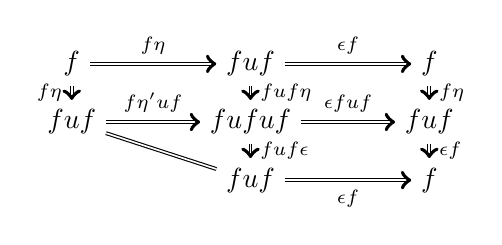
\begin{tikzpicture}[x=1.7em,y=1.4em]
  \node (f1)    at (0,1.5)     {$f$};
  \node (fuf1)  at (3.8,1.5)   {$fuf$};
  \node (f2)    at (7.6,1.5)   {$f$};
  \node (fuf2)  at (0,0)       {$fuf$};
  \node (fufuf) at (3.8,0)     {$fufuf$};
  \node (fuf3)  at (7.6,0)     {$fuf$};
  \node (fuf4)  at (3.8,-1.5)  {$fuf$};
  \node (f3)    at (7.6,-1.5)  {$f$};
  \draw[double,->] (f1) -- node[above]{$\scriptstyle f\eta$} (fuf1);
  \draw[double,->] (fuf1) -- node[above]{$\scriptstyle\epsilon f$} (f2);
  \draw[double,->] (f1) -- node[left]{$\scriptstyle f\eta$} (fuf2);
  \draw[double,->] (fuf1) -- node[right]{$\scriptstyle fuf\eta$} (fufuf);
  \draw[double,->] (fufuf) -- node[right]{$\scriptstyle fuf\epsilon$} (fuf4);
  \draw[double,->] (f2) -- node[right]{$\scriptstyle f\eta$} (fuf3);
  \draw[double,->] (fuf3) -- node[right]{$\scriptstyle\epsilon f$} (f3);
  \draw[double,->] (fuf2) -- node[above]{$\scriptstyle f\eta' uf$} (fufuf);
  \draw[double,->] (fufuf) -- node[above]{$\scriptstyle\epsilon fuf$} (fuf3);
  \draw[double,->] (fuf4) -- node[below]{$\scriptstyle\epsilon f$} (f3);
  \draw[double] (fuf2) -- (fuf4);
\end{tikzpicture}
\end{center}
由消去法，任何\trIdempotent{}同构都是恒等，这就证得
$\epsilon f\cdot f\eta=\mathrm{id}_{f}$。
\end{proof}

一个\trGeneralizedElement{} $y\colon z\to b$ 被称为属于一支 1-\trCell{}
$u\colon a\to b$ 的\textbf{本质像}（essential image），若存在一个\trGeneralizedElement{}
$x\colon z\to a$ 与一个可逆 2-\trCell{} $\beta\colon y\cong ux$。当\trFunctor{} $u$ 是
$f$ 的\trRightAdjoint\trRightInverse{}时，其本质像有一个便利的刻画：

\begin{lemma}\label{lem:rajri-essential-image}
一个\trGeneralizedElement{} $y\colon z\to b$ 属于\trRightAdjoint\trRightInverse{}
$u\colon a\to b$ 的本质像，当且仅当\trUnit{}分量 $\eta y\colon y\Rightarrow ufy$ 是一个%
\trIsomorphism。
\end{lemma}

\begin{proof}
尚需论证的只是：若给定一个可逆 2-\trCell{} $\beta\colon y\cong ux$，则\trUnit{}分量
$\eta y$ 也是一个\trIsomorphism。这由\cref{lem:naturality-of-whiskering}那条平凡的末尾
论断即得。从左下方那对可水平复合的 2-\trCell{}出发，\trWhiskering{}的自然性给出右下方
的交换图表：
\begin{center}
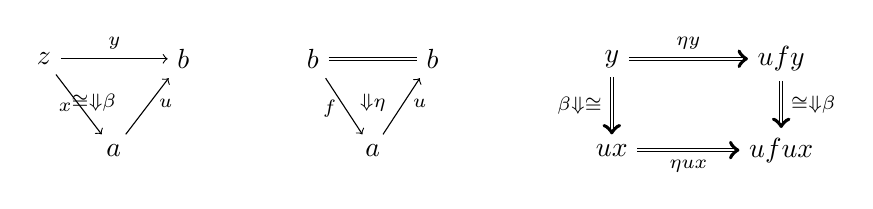
\begin{tikzpicture}[x=1.8em,y=1.5em]
  \node (z) at (0,1.1)    {$z$};
  \node (b) at (2.8,1.1)  {$b$};
  \node (a) at (1.4,-1.1) {$a$};
  \draw[->] (z) -- node[above]{$\scriptstyle y$} (b);
  \draw[->] (z) -- node[left,pos=0.55]{$\scriptstyle x$} (a);
  \draw[->] (a) -- node[right,pos=0.55]{$\scriptstyle u$} (b);
  \node at (1.0,0.05) {$\scriptstyle\cong\Downarrow\beta$};
  \node (b2) at (5.4,1.1)  {$b$};
  \node (b3) at (7.8,1.1)  {$b$};
  \node (a2) at (6.6,-1.1) {$a$};
  \draw[double] (b2) -- (b3);
  \draw[->] (b2) -- node[left,pos=0.55]{$\scriptstyle f$} (a2);
  \draw[->] (a2) -- node[right,pos=0.55]{$\scriptstyle u$} (b3);
  \node at (6.6,0.05) {$\scriptstyle\Downarrow\eta$};
  \node at (9.2,0) {$\rightsquigarrow$};
  \node (y)    at (11.4,1.1)  {$y$};
  \node (ufy)  at (14.8,1.1)  {$ufy$};
  \node (ux)   at (11.4,-1.1) {$ux$};
  \node (ufux) at (14.8,-1.1) {$ufux$};
  \draw[double,->] (y) -- node[above]{$\scriptstyle\eta y$} (ufy);
  \draw[double,->] (y) -- node[left]{$\scriptstyle\beta\Downarrow\cong$} (ux);
  \draw[double,->] (ufy) -- node[right]{$\scriptstyle\cong\Downarrow\beta$} (ufux);
  \draw[double,->] (ux) -- node[below]{$\scriptstyle\eta ux$} (ufux);
\end{tikzpicture}
\end{center}
由于 $u$ 是\trRightAdjoint\trRightInverse，$\eta u$ 可逆。于是，若 $\beta$ 可逆，则
$\eta y$ 亦可逆。
\end{proof}

有时，使用一种更严格的右伴随右逆伴随概念会更加方便，其中\trCounit{} $\epsilon$ 被要求
是恒等式 $fu=\mathrm{id}_{a}$。在这种情形下，由\trTriangleEqualities{}可得
$f\eta=\mathrm{id}_{f}$，从而\trUnit{}纤维化于 $a$ 之上。当\trLeftAdjoint{}在下述
2-范畴意义下是一个\trIsofibration{}时，同构意义下的右伴随右逆总可以替换为恒等意义下的
右伴随右逆（见第 3 章中的\cref{lem:rajri-fibered-adjunction}）。

\begin{definition}[等价纤维化]\label{def:rajri-isofibration}
2-\trCategory{}中的一支 1-\trCell{} $f\colon b\to a$ 定义一个%
\textbf{\trIsofibration}——此时该箭头通常记作「$\twoheadrightarrow$」——若给定任何
抵接于 $a$ 的可逆 2-\trCell{} $\alpha\colon fy\cong x$，连同其\trBoundary{} 1-\trCell{}%
之一穿过 $f$ 的一个指定提升，则存在抵接于 $b$ 的可逆 2-\trCell{}
$\beta\colon y\cong\bar{y}$ 带有这一\trBoundary{} 1-\trCell，它与 $f$ 须化后等于原先的
2-\trCell：
\begin{center}
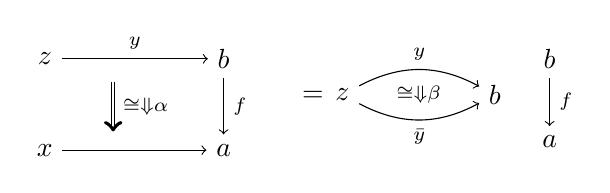
\begin{tikzpicture}[x=1.9em,y=1.5em]
  \node (z) at (0,0.9)    {$z$};
  \node (b) at (3.4,0.9)  {$b$};
  \node (xt) at (0,-1.3)  {$x$};
  \node (a) at (3.4,-1.3) {$a$};
  \draw[->] (z) -- node[above]{$\scriptstyle y$} (b);
  \draw[->] (b) -- node[right]{$\scriptstyle f$} (a);
  \draw[->] (xt) -- (a);
  \draw[double,->] (1.3,0.35) -- node[right]{$\scriptstyle\cong\Downarrow\alpha$}
    (1.3,-0.85);
  \node at (5.1,0) {$=$};
  \node at (7.1,0) {\hTwoCell{z}{b}{y}{\,\cong\Downarrow\beta\,}{\bar{y}}};
  \node (fb) at (9.6,0.9)  {$b$};
  \node (fa) at (9.6,-1.1) {$a$};
  \draw[->] (fb) -- node[right]{$\scriptstyle f$} (fa);
\end{tikzpicture}
\end{center}
\end{definition}

\begin{lemma}\label{lem:rajri-isofibration}
设 $f\colon b\twoheadrightarrow a$ 是 2-\trCategory{} $\mathcal{C}$ 中任何一支容许%
\trRightAdjoint{} $u'\colon a\to b$ 的\trIsofibration，其\trCounit{}
$\epsilon\colon fu'\cong\mathrm{id}_{a}$ 是一个\trIsomorphism。则 $u'$
\trIsomorphism{}于一个严格位于 $a$ 之上的\trFunctor{} $u$，后者定义了 $f$ 的一个严格右
伴随右逆，此时 $f\dashv u$ 在 2-\trCategory{} $\mathcal{C}_{/a}$——由以 $a$ 为余定义域
的\trIsofibration、$a$ 之上的交换三角形以及经须化后成为抵接于 $a$ 的恒等的
2-\trCell{}组成——中定义一个\trAdjunction。
\end{lemma}

\begin{center}
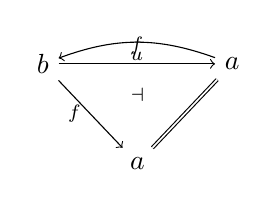
\begin{tikzpicture}[x=1.9em,y=1.5em]
  \node (b)  at (0,1.2)    {$b$};
  \node (a)  at (3.6,1.2)  {$a$};
  \node (a2) at (1.8,-1.2) {$a$};
  \draw[->] (b) -- node[above]{$\scriptstyle f$} (a);
  \draw[->] (a) to[bend right=20] node[below,pos=0.5]{$\scriptstyle u$} (b);
  \node at (1.8,0.45) {$\scriptstyle\dashv$};
  \draw[->] (b) -- node[left,pos=0.5]{$\scriptstyle f$} (a2);
  \draw[double] (a2) -- (a);
\end{tikzpicture}
\end{center}

\begin{proof}
将\trCounit{}同构经由\trIsofibration{} $f\colon b\twoheadrightarrow a$ 提升，由此定义
1-\trCell{} $u\colon a\to b$：
\begin{center}
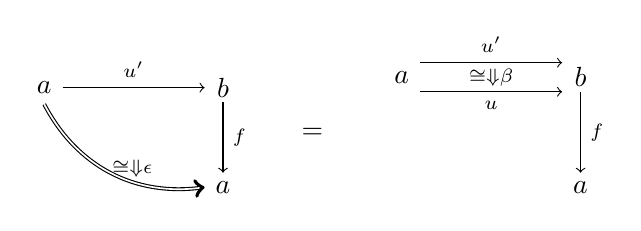
\begin{tikzpicture}[x=1.9em,y=1.5em]
  \node (la)  at (0,1.1)    {$a$};
  \node (lb)  at (3.4,1.1)  {$b$};
  \node (la2) at (3.4,-1.3) {$a$};
  \draw[->] (0.35,1.1) -- node[above]{$\scriptstyle u'$} (3.05,1.1);
  \draw[->] (3.4,0.75) -- node[right]{$\scriptstyle f$} (3.4,-0.95);
  \draw[double,->] (0,0.7) to[bend right=35]
    node[right,pos=0.45]{$\scriptstyle\cong\Downarrow\epsilon$} (3.05,-1.3);
  \node at (5.1,0) {$=$};
  \node (ra)  at (6.8,1.35)  {$a$};
  \node (rb)  at (10.2,1.35) {$b$};
  \node (ra2) at (10.2,-1.3) {$a$};
  \draw[->] (7.15,1.7) -- node[above]{$\scriptstyle u'$} (9.85,1.7);
  \draw[->] (7.15,1.0) -- node[below]{$\scriptstyle u$} (9.85,1.0);
  \node at (8.5,1.35) {$\scriptstyle\cong\Downarrow\beta$};
  \draw[->] (10.2,1.0) -- node[right]{$\scriptstyle f$} (10.2,-0.95);
\end{tikzpicture}
\end{center}
由构造即知 $fu=\mathrm{id}_{a}$，故 $u$ 定义了 $\mathcal{C}_{/a}$ 中的一个 1-\trCell。
由\trAdjunction{} $f\dashv u'$ 的\trTriangleEqualities，其\trUnit{}定义了一个
2-\trCell{} $\eta\colon\mathrm{id}_{b}\Rightarrow u'f$，其中 $\eta u'$ 与 $f\eta$ 均
可逆。复合 2-\trCell
\[
\eta' \coloneqq \mathrm{id}_{b} \xRightarrow{\;\eta\;} u'f
  \xRightarrow[\;\cong\;]{\;\beta f\;} uf
\]
位于 $\mathcal{C}_{/a}$ 中，且具有 $\eta'u$ 与 $f\eta$ 均可逆之性质。在 2-\trCategory{}
$\mathcal{C}_{/a}$ 中应用\cref{lem:rajri-modification}，这条 2-\trCell{}随后便可经修改
而定义一个\trAdjunction{} $f\dashv u$ 的\trUnit，其\trCounit{}满足 $fu=\mathrm{id}_{a}$。
\end{proof}

\subsection*{练习}

\begin{exercise}\label{ex:rajri-equivalent-adjunctions}
考虑一对等价的\trAdjunction，满足\cref{prop:equivalence-invariance-of-adjointness}的
条件。证明：若其中任一个是\trRightAdjoint\trRightInverse\trAdjunction，则二者皆是。
\end{exercise}

   %

\providecommand{\Cat}{\mathcal{C}at}

\section{绝对绝对提升图}\label{sec:absolute-absolute-lifting-diagrams}

回忆第 2 章中的\cref{def:absolute-left-lifting}：对 2-\trCategory{}中任意%
\trCospan{} $c\xrightarrow{g}a\xleftarrow{f}b$，$g$ 沿 $f$ 的一个%
\textbf{绝对右\trLifting}由
一支 1-\trCell{} $r$ 与一个 2-\trCell{} $\rho$ 给出，如下左图所示：
\begin{center}
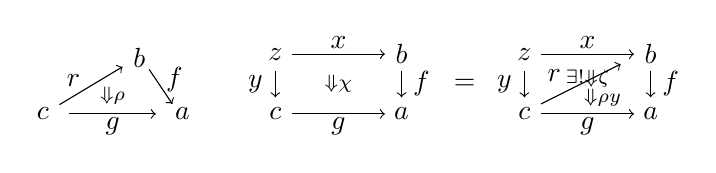
\begin{tikzpicture}[x=1.2em,y=1.2em]
  \node (c1) at (0,0) {$c$};
  \node (a1) at (4.2,0) {$a$};
  \node (b1) at (2.9,1.7) {$b$};
  \draw[->] (0.5,0.28) -- (2.4,1.42);
  \node at (0.92,1.02) {$r$};
  \draw[->] (3.2,1.34) -- (3.9,0.3);
  \node at (3.96,1.02) {$f$};
  \draw[->] (0.8,0) -- (3.4,0);
  \node at (2.1,-0.38) {$g$};
  \node at (2.1,0.55) {$\scriptstyle\Downarrow\rho$};
  \node (z2) at (7.0,1.8) {$z$};
  \node (b2) at (10.8,1.8) {$b$};
  \node (c2) at (7.0,0) {$c$};
  \node (a2) at (10.8,0) {$a$};
  \draw[->] (7.5,1.8) -- (10.3,1.8);
  \node at (8.9,2.14) {$x$};
  \draw[->] (10.8,1.3) -- (10.8,0.5);
  \node at (11.4,0.9) {$f$};
  \draw[->] (7.0,1.3) -- (7.0,0.5);
  \node at (6.4,0.9) {$y$};
  \draw[->] (7.5,0) -- (10.3,0);
  \node at (8.9,-0.38) {$g$};
  \node at (8.9,0.9) {$\scriptstyle\Downarrow\chi$};
  \node at (12.7,0.9) {$=$};
  \node (z3) at (14.5,1.8) {$z$};
  \node (b3) at (18.3,1.8) {$b$};
  \node (c3) at (14.5,0) {$c$};
  \node (a3) at (18.3,0) {$a$};
  \draw[->] (15.0,1.8) -- (17.8,1.8);
  \node at (16.4,2.14) {$x$};
  \draw[->] (18.3,1.3) -- (18.3,0.5);
  \node at (18.9,0.9) {$f$};
  \draw[->] (14.5,1.3) -- (14.5,0.5);
  \node at (13.9,0.9) {$y$};
  \draw[->] (15.0,0) -- (17.8,0);
  \node at (16.4,-0.38) {$g$};
  \draw[->] (15.0,0.3) -- (17.4,1.5);
  \node at (15.4,1.16) {$r$};
  \node at (16.4,1.05) {$\scriptstyle\exists!\Downarrow\zeta$};
  \node at (16.85,0.5) {$\scriptstyle\Downarrow\rho y$};
\end{tikzpicture}
\end{center}
从而，任何如中图所示的 2-\trCell{}都能唯一地经由 $(r,\rho)$ 分解成如右图所示的
形状。「绝对」这一形容词指的是如下性质：绝对右\trLifting{}图在沿任何
1-\trCell{} $k\colon d\to c$ 作限制下稳定。

下面这条引理给出第二重意义下为绝对的绝对右\trLifting{}图：亦即，它们被任何%
\trTwoFunctor{}保持。

\begin{lemma}\label{lem:absolute-lifting-under-adjunction}
设有\emph{在 $b$ 之下的}\trAdjunction{}（$f\dashv u$、$\eta\colon\mathrm{id}_{a}\Rightarrow uf$、
$\epsilon\colon fu\Rightarrow\mathrm{id}_{c}$），其意义如下：
\begin{itemize}
\item 涉及两个\trAdjunction{}的实箭头三角形均交换
\begin{center}
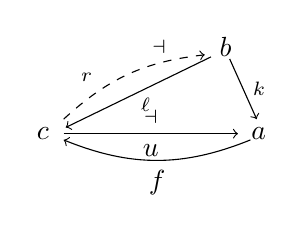
\begin{tikzpicture}[x=1.5em,y=1.5em]
  \node (b) at (4.4,2.1) {$b$};
  \node (c) at (0,0) {$c$};
  \node (a) at (5.2,0) {$a$};
  \draw[->,dashed] (0.5,0.35) to[bend left=18]
    node[pos=0.72,above]{$\scriptstyle\dashv$} (3.9,1.9);
  \node at (1.05,1.35) {$\scriptstyle r$};
  \draw[->] (4.05,1.85) -- node[below,pos=0.45]{$\scriptstyle\ell$} (0.55,0.15);
  \draw[->] (4.5,1.8) -- node[right,pos=0.5]{$\scriptstyle k$} (5.15,0.35);
  \draw[->] (0.5,0) -- (4.7,0);
  \node at (2.6,0.4) {$\scriptstyle\dashv$};
  \node at (2.6,-0.4) {$u$};
  \draw[->] (5.0,-0.15) to[bend left=22] node[below,pos=0.5]{$f$} (0.5,-0.15);
\end{tikzpicture}
\end{center}
\item 并且 $\eta k=\mathrm{id}_{k}$ 且 $\epsilon\ell=\mathrm{id}_{\ell}$。
\end{itemize}
此时，若 $\ell$ 容许一个\trRightAdjoint{} $r$，其\trUnit{}为
$\iota\colon\mathrm{id}_{b}\Rightarrow r\ell$、\trCounit{}为
$\nu\colon\ell r\Rightarrow\mathrm{id}_{c}$，则 $u\nu$ 展示 $r$ 为 $u$ 沿 $k$
的一个绝对右\trLifting{}：
\begin{center}
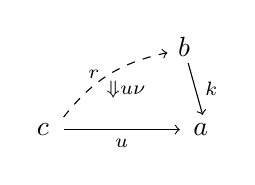
\begin{tikzpicture}[x=1.5em,y=1.5em]
  \node (b) at (3.4,2.0) {$b$};
  \node (c) at (0,0) {$c$};
  \node (a) at (3.8,0) {$a$};
  \draw[->,dashed] (0.5,0.3) to[bend left=20]
    node[left,pos=0.5]{$\scriptstyle r$} (3.0,1.85);
  \draw[->] (3.5,1.6) -- node[right]{$\scriptstyle k$} (3.85,0.35);
  \draw[->] (0.5,0) -- node[below]{$\scriptstyle u$} (3.3,0);
  \node at (2.0,0.95) {$\scriptstyle\Downarrow u\nu$};
\end{tikzpicture}
\end{center}
此外，这类绝对右\trLifting{}图被任何\trTwoFunctor{}保持。
\end{lemma}

\begin{proof}
论证是纯图解式的：任何如下左图所示的 2-\trCell{}都经由 $u\nu$ 分解，正如下图
链所展示的那样：
\begin{center}
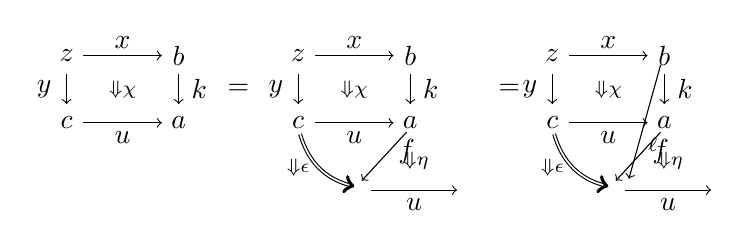
\begin{tikzpicture}[x=1.35em,y=1.35em]
  \node (z1) at (0,1.8) {$z$};
  \node (b1) at (3.0,1.8) {$b$};
  \node (c1) at (0,0) {$c$};
  \node (a1) at (3.0,0) {$a$};
  \draw[->] (0.45,1.8) -- (2.55,1.8);
  \node at (1.5,2.14) {$x$};
  \draw[->] (3.0,1.3) -- (3.0,0.5);
  \node at (3.55,0.9) {$k$};
  \draw[->] (0,1.3) -- (0,0.5);
  \node at (-0.6,0.9) {$y$};
  \draw[->] (0.45,0) -- (2.55,0);
  \node at (1.5,-0.4) {$u$};
  \node at (1.5,0.9) {$\scriptstyle\Downarrow\chi$};
  \node at (4.6,0.9) {$=$};
  \node (z2) at (6.2,1.8) {$z$};
  \node (b2) at (9.2,1.8) {$b$};
  \node (c2) at (6.2,0) {$c$};
  \node (a2) at (9.2,0) {$a$};
  \draw[->] (6.65,1.8) -- (8.75,1.8);
  \node at (7.7,2.14) {$x$};
  \draw[->] (9.2,1.3) -- (9.2,0.5);
  \node at (9.75,0.9) {$k$};
  \draw[->] (6.2,1.3) -- (6.2,0.5);
  \node at (5.6,0.9) {$y$};
  \draw[->] (6.65,0) -- (8.75,0);
  \node at (7.7,-0.4) {$u$};
  \node at (7.7,0.9) {$\scriptstyle\Downarrow\chi$};
  \draw[->] (9.1,-0.25) -- node[right,pos=0.4]{$f$} (7.9,-1.55);
  \node at (9.35,-1.0) {$\scriptstyle\Downarrow\eta$};
  \draw[->,double] (6.25,-0.3) to[bend right=30]
    node[left,pos=0.5]{$\scriptstyle\Downarrow\epsilon$} (7.7,-1.7);
  \draw[->] (8.15,-1.8) -- (10.45,-1.8);
  \node at (9.3,-2.2) {$u$};
  \node at (11.85,0.9) {$=$};
  \node (z3) at (13.0,1.8) {$z$};
  \node (b3) at (16.0,1.8) {$b$};
  \node (c3) at (13.0,0) {$c$};
  \node (a3) at (16.0,0) {$a$};
  \draw[->] (13.45,1.8) -- (15.55,1.8);
  \node at (14.5,2.14) {$x$};
  \draw[->] (16.0,1.3) -- (16.0,0.5);
  \node at (16.55,0.9) {$k$};
  \draw[->] (13.0,1.3) -- (13.0,0.5);
  \node at (12.4,0.9) {$y$};
  \draw[->] (13.45,0) -- (15.55,0);
  \node at (14.5,-0.4) {$u$};
  \node at (14.5,0.9) {$\scriptstyle\Downarrow\chi$};
  \draw[->] (15.9,-0.25) -- node[right,pos=0.4]{$f$} (14.7,-1.55);
  \node at (16.15,-1.0) {$\scriptstyle\Downarrow\eta$};
  \draw[->,double] (13.05,-0.3) to[bend right=30]
    node[left,pos=0.5]{$\scriptstyle\Downarrow\epsilon$} (14.5,-1.7);
  \draw[->] (14.95,-1.8) -- (17.25,-1.8);
  \node at (16.1,-2.2) {$u$};
  \draw[->] (15.9,1.55) -- node[right,pos=0.7]{$\scriptstyle\ell$} (15.05,-1.5);
\end{tikzpicture}
\end{center}
\begin{center}
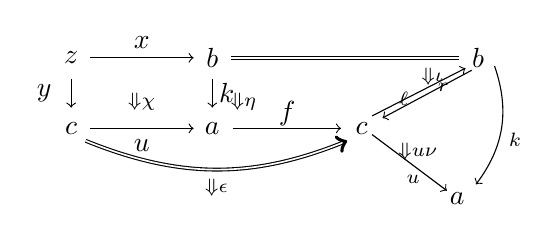
\begin{tikzpicture}[x=1.5em,y=1.5em]
  \node (z)  at (0,3.4)  {$z$};
  \node (b1) at (3.4,3.4) {$b$};
  \node (b2) at (9.8,3.4) {$b$};
  \draw[double] (3.85,3.4) -- (9.35,3.4);
  \node (c)  at (0,1.7)  {$c$};
  \node (a)  at (3.4,1.7) {$a$};
  \node (c2) at (7.0,1.7) {$c$};
  \node (a3) at (9.3,0)  {$a$};
  \draw[->] (0.45,3.4) -- (2.95,3.4);
  \node at (1.7,3.76) {$x$};
  \draw[->] (0,2.9) -- (0,2.2);
  \node at (-0.65,2.55) {$y$};
  \draw[->] (3.4,2.9) -- (3.4,2.2);
  \node at (3.75,2.55) {$k$};
  \draw[->] (0.45,1.7) -- (2.95,1.7);
  \node at (1.7,1.28) {$u$};
  \node at (1.7,2.35) {$\scriptstyle\Downarrow\chi$};
  \draw[->] (3.9,1.7) -- (6.5,1.7);
  \node at (5.2,2.06) {$f$};
  \node at (4.15,2.35) {$\scriptstyle\Downarrow\eta$};
  \draw[->,double] (0.35,1.4) to[bend right=22]
    node[below,pos=0.5]{$\scriptstyle\Downarrow\epsilon$} (6.65,1.4);
  \draw[->] (7.25,2.0) -- node[right,pos=0.6]{$\scriptstyle r$} (9.5,3.15);
  \draw[->] (9.65,3.1) -- node[left,pos=0.6]{$\scriptstyle\ell$} (7.5,1.95);
  \node at (8.7,2.95) {$\scriptstyle\Downarrow\iota$};
  \draw[->] (10.2,3.2) to[bend left=28] node[right,pos=0.6]{$\scriptstyle k$} (9.75,0.35);
  \draw[->] (7.25,1.55) -- node[below,pos=0.55]{$\scriptstyle u$} (9.05,0.2);
  \node at (8.35,1.15) {$\scriptstyle\Downarrow u\nu$};
\end{tikzpicture}
\end{center}

反之，若 $\zeta$ 给出 $\chi$ 经由 $u\nu$ 的一个分解，则
\begin{center}
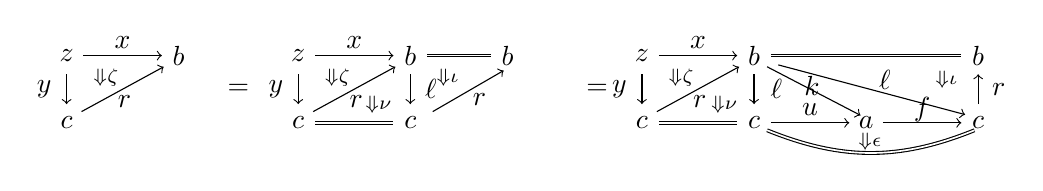
\begin{tikzpicture}[x=1.35em,y=1.35em]
  \node (z4) at (0,1.8) {$z$};
  \node (b4) at (3.0,1.8) {$b$};
  \node (c4) at (0,0) {$c$};
  \draw[->] (0.45,1.8) -- (2.55,1.8);
  \node at (1.5,2.14) {$x$};
  \draw[->] (0,1.3) -- (0,0.5);
  \node at (-0.6,0.9) {$y$};
  \draw[->] (0.4,0.3) -- (2.6,1.5);
  \node at (1.55,0.58) {$r$};
  \node at (1.05,1.22) {$\scriptstyle\Downarrow\zeta$};
  \node at (4.6,0.9) {$=$};
  \node (z5) at (6.2,1.8) {$z$};
  \node (b5) at (9.2,1.8) {$b$};
  \node (b6) at (11.8,1.8) {$b$};
  \draw[double] (9.65,1.8) -- (11.35,1.8);
  \node (c5) at (6.2,0) {$c$};
  \node (c6) at (9.2,0) {$c$};
  \draw[double] (6.65,0) -- (8.75,0);
  \draw[->] (6.65,1.8) -- (8.75,1.8);
  \node at (7.7,2.14) {$x$};
  \draw[->] (6.2,1.3) -- (6.2,0.5);
  \node at (5.6,0.9) {$y$};
  \draw[->] (6.6,0.3) -- (8.8,1.5);
  \node at (7.75,0.58) {$r$};
  \node at (7.25,1.22) {$\scriptstyle\Downarrow\zeta$};
  \node at (8.35,0.48) {$\scriptstyle\Downarrow\nu$};
  \draw[->] (9.2,1.3) -- (9.2,0.5);
  \node at (9.75,0.9) {$\ell$};
  \draw[->] (9.8,0.3) -- (11.7,1.4);
  \node at (11.05,0.62) {$r$};
  \node at (10.2,1.22) {$\scriptstyle\Downarrow\iota$};
  \node at (14.2,0.9) {$=$};
  \node (z6) at (15.4,1.8) {$z$};
  \node (b7) at (18.4,1.8) {$b$};
  \node (b8) at (24.4,1.8) {$b$};
  \draw[double] (18.85,1.8) -- (23.95,1.8);
  \node (c7) at (15.4,0) {$c$};
  \node (c8) at (18.4,0) {$c$};
  \node (a4) at (21.4,0) {$a$};
  \node (c9) at (24.4,0) {$c$};
  \draw[->] (15.85,1.8) -- (17.95,1.8);
  \node at (16.9,2.14) {$x$};
  \draw[->] (15.4,1.3) -- (15.4,0.5);
  \node at (14.8,0.9) {$y$};
  \draw[->] (15.8,0.3) -- (18.0,1.5);
  \node at (16.95,0.58) {$r$};
  \node at (16.45,1.22) {$\scriptstyle\Downarrow\zeta$};
  \node at (17.6,0.48) {$\scriptstyle\Downarrow\nu$};
  \draw[double] (15.85,0) -- (17.95,0);
  \draw[->] (18.4,1.3) -- (18.4,0.5);
  \node at (19.0,0.9) {$\ell$};
  \draw[->] (18.85,0) -- (20.95,0);
  \node at (19.9,0.36) {$u$};
  \draw[->] (21.85,0) -- (23.95,0);
  \node at (22.9,0.36) {$f$};
  \draw[->] (18.75,1.5) -- (21.25,0.2);
  \node at (19.95,0.98) {$k$};
  \draw[->] (19.05,1.55) -- (24.05,0.22);
  \node at (21.9,1.15) {$\ell$};
  \node at (23.55,1.15) {$\scriptstyle\Downarrow\iota$};
  \draw[->] (24.4,0.5) -- (24.4,1.3);
  \node at (24.95,0.9) {$r$};
  \draw[double] (18.75,-0.2) to[bend right=22] (24.3,-0.2);
  \node at (21.5,-0.5) {$\scriptstyle\Downarrow\epsilon$};
\end{tikzpicture}
\end{center}
\begin{center}
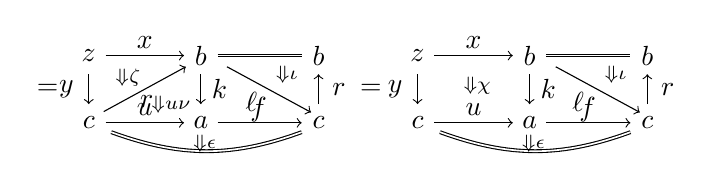
\begin{tikzpicture}[x=1.35em,y=1.35em]
  \node at (-1.1,0.9) {$=$};
  \node (z7) at (0,1.8) {$z$};
  \node (b9) at (3.0,1.8) {$b$};
  \node (b10) at (6.15,1.8) {$b$};
  \draw[double] (3.45,1.8) -- (5.7,1.8);
  \node (c10) at (0,0) {$c$};
  \node (a5) at (3.0,0) {$a$};
  \node (c11) at (6.15,0) {$c$};
  \draw[->] (0.45,1.8) -- (2.55,1.8);
  \node at (1.5,2.14) {$x$};
  \draw[->] (0,1.3) -- (0,0.5);
  \node at (-0.6,0.9) {$y$};
  \draw[->] (0.4,0.3) -- (2.6,1.5);
  \node at (1.55,0.58) {$r$};
  \node at (1.05,1.22) {$\scriptstyle\Downarrow\zeta$};
  \node at (2.2,0.48) {$\scriptstyle\Downarrow u\nu$};
  \draw[->] (3.0,1.3) -- (3.0,0.5);
  \node at (3.5,0.9) {$k$};
  \draw[->] (3.7,1.5) -- (5.95,0.28);
  \node at (4.35,0.55) {$\ell$};
  \node at (5.3,1.3) {$\scriptstyle\Downarrow\iota$};
  \draw[->] (6.15,0.5) -- (6.15,1.3);
  \node at (6.7,0.9) {$r$};
  \draw[->] (0.45,0) -- (2.55,0);
  \node at (1.5,0.36) {$u$};
  \draw[->] (3.45,0) -- (5.7,0);
  \node at (4.55,0.36) {$f$};
  \draw[double] (0.6,-0.25) to[bend right=20] (5.7,-0.25);
  \node at (3.1,-0.55) {$\scriptstyle\Downarrow\epsilon$};
  \node at (7.55,0.9) {$=$};
  \node (z8) at (8.8,1.8) {$z$};
  \node (b11) at (11.8,1.8) {$b$};
  \node (b12) at (14.95,1.8) {$b$};
  \draw[double] (12.25,1.8) -- (14.5,1.8);
  \node (c12) at (8.8,0) {$c$};
  \node (a6) at (11.8,0) {$a$};
  \node (c13) at (14.95,0) {$c$};
  \draw[->] (9.25,1.8) -- (11.35,1.8);
  \node at (10.3,2.14) {$x$};
  \draw[->] (8.8,1.3) -- (8.8,0.5);
  \node at (8.2,0.9) {$y$};
  \node at (10.4,1.0) {$\scriptstyle\Downarrow\chi$};
  \draw[->] (11.8,1.3) -- (11.8,0.5);
  \node at (12.3,0.9) {$k$};
  \draw[->] (12.5,1.5) -- (14.75,0.28);
  \node at (13.1,0.55) {$\ell$};
  \node at (14.1,1.3) {$\scriptstyle\Downarrow\iota$};
  \draw[->] (14.95,0.5) -- (14.95,1.3);
  \node at (15.5,0.9) {$r$};
  \draw[->] (9.25,0) -- (11.35,0);
  \node at (10.3,0.36) {$u$};
  \draw[->] (12.25,0) -- (14.5,0);
  \node at (13.35,0.36) {$f$};
  \draw[double] (9.4,-0.25) to[bend right=20] (14.5,-0.25);
  \node at (11.9,-0.55) {$\scriptstyle\Downarrow\epsilon$};
\end{tikzpicture}
\end{center}
这就证明了上文所构造的分解是唯一的。最后，由于绝对右\trLifting{}图的%
\trUniversalProperty{}由诸
伴随的存在所「以等式方式见证」，故它被任何\trTwoFunctor{}保持。
\end{proof}

\begin{example}\label{exa:delta-adjoint-diagram}
例如，存在由\trAdjunction{}\trFunctor{}构成的如下\trDiagram
\begin{center}
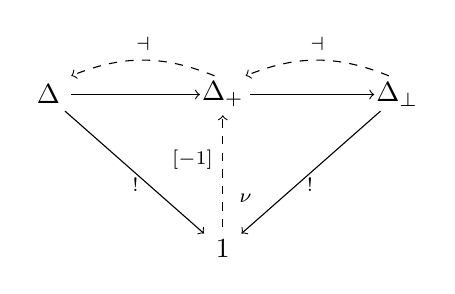
\begin{tikzpicture}[x=1.5em,y=1.5em]
  \node (D)  at (0,2.2)  {$\Delta$};
  \node (Dp) at (4.2,2.2) {$\Delta_{+}$};
  \node (Db) at (8.4,2.2) {$\Delta_{\perp}$};
  \draw[->] (0.55,2.2) -- (3.65,2.2);
  \draw[->] (4.85,2.2) -- (7.85,2.2);
  \draw[->,dashed] (4.0,2.65) to[bend right=22]
    node[above,pos=0.5]{$\scriptstyle\dashv$} (0.55,2.65);
  \draw[->,dashed] (8.2,2.65) to[bend right=22]
    node[above,pos=0.5]{$\scriptstyle\dashv$} (4.75,2.65);
  \node (one) at (4.2,-1.5) {$1$};
  \draw[->] (0.4,1.8) -- node[left,pos=0.6]{$\scriptstyle!$} (3.75,-1.15);
  \draw[->] (8.0,1.8) -- node[right,pos=0.6]{$\scriptstyle!$} (4.65,-1.15);
  \draw[->,dashed] (4.2,-1.0) -- node[left,pos=0.6]{$\scriptstyle[-1]$} (4.2,1.7);
  \node at (4.75,-0.3) {$\scriptstyle\nu$};
\end{tikzpicture}
\end{center}
它涉及第 2 章中的\cref{def:split-augmented}所引入的那些\trCategory{}。包含
$\Delta\hookrightarrow\Delta_{+}\hookrightarrow\Delta_{\perp}$ 自由地为每个序数
添入一个底元素，而其\trRightAdjoint{}则可等同于宽子范畴（其态射皆为保持底元素
的映射）的包含 $\Delta_{\perp}\hookrightarrow\Delta$。\trAdjunction{}
$[-1]\dashv\,!$ 见证
了下述事实：$[-1]\in\Delta_{\perp}$ 定义一个\trInitial{}对象，其\trCounit{} $\nu$
给出从该\trInitial{}对象到恒同\trFunctor{}的典范\trNaturalTransformation。这一%
\trDiagram{}在 $\Cat^{\mathrm{op}}$ 中满足\cref{lem:absolute-lifting-under-adjunction}的
前提。设 $a$ 为任一在 $\Cat$ 上\trCotensor{}的 2-\trCategory{} $\mathcal{C}$ 中的
一个对象，则 2-\trFunctor{} $a^{(-)}\colon\Cat^{\mathrm{op}}\to\mathcal{C}$ 把所给
数据携带为 $\mathcal{C}$ 中如下左图所示的\trAdjunction{}\trFunctor{}\trDiagram，从而如下右图所示
的三角形是一个绝对右\trLifting{}：
\begin{center}
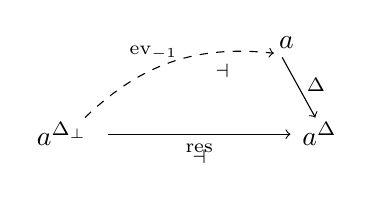
\begin{tikzpicture}[x=1.5em,y=1.5em]
  \node (aL)  at (5.4,2.2) {$a$};
  \node (aDbL) at (0,0) {$a^{\Delta_{\perp}}$};
  \node (aDL) at (6.2,0) {$a^{\Delta}$};
  \draw[->,dashed] (0.55,0.4) to[bend left=25]
    node[above,pos=0.4]{$\scriptstyle\mathrm{ev}_{-1}$}
    node[pos=0.68,below right]{$\scriptstyle\dashv$} (5.1,1.95);
  \draw[->] (5.3,1.85) -- node[right,pos=0.45]{$\scriptstyle\Delta$} (6.1,0.4);
  \draw[->] (1.1,0) -- node[below]{$\scriptstyle\mathrm{res}$} (5.5,0);
  \node at (3.3,-0.55) {$\scriptstyle\dashv$};
\end{tikzpicture}
\qquad
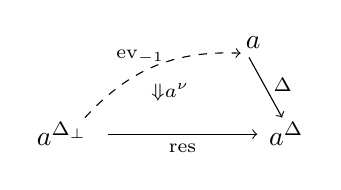
\begin{tikzpicture}[x=1.5em,y=1.5em]
  \node (aR)  at (4.6,2.2) {$a$};
  \node (aDbR) at (0,0) {$a^{\Delta_{\perp}}$};
  \node (aDR) at (5.4,0) {$a^{\Delta}$};
  \draw[->,dashed] (0.55,0.4) to[bend left=25]
    node[above,pos=0.4]{$\scriptstyle\mathrm{ev}_{-1}$} (4.3,1.95);
  \draw[->] (4.5,1.85) -- node[right,pos=0.45]{$\scriptstyle\Delta$} (5.3,0.4);
  \draw[->] (1.1,0) -- node[below]{$\scriptstyle\mathrm{res}$} (4.7,0);
  \node at (2.6,1.0) {$\scriptstyle\Downarrow a^{\nu}$};
\end{tikzpicture}
\end{center}
这就证明了第 2 章中的\cref{prop:split-limits}。
\end{example}

\begin{example}\label{exa:top-splitting-adjunctions}
存在一幅类似的由\trAdjunction{}\trFunctor{}构成的如下\trDiagram
\begin{center}
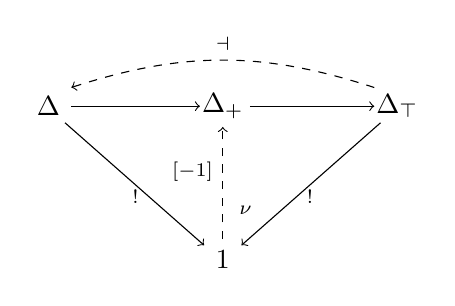
\begin{tikzpicture}[x=1.5em,y=1.5em]
  \node (D)  at (0,2.2)  {$\Delta$};
  \node (Dp) at (4.2,2.2) {$\Delta_{+}$};
  \node (Dt) at (8.4,2.2) {$\Delta_{\top}$};
  \draw[->] (0.55,2.2) -- (3.65,2.2);
  \draw[->] (4.85,2.2) -- (7.85,2.2);
  \draw[->,dashed] (7.85,2.65) to[bend right=18]
    node[above,pos=0.5]{$\scriptstyle\dashv$} (0.55,2.65);
  \node (one) at (4.2,-1.5) {$1$};
  \draw[->] (0.4,1.8) -- node[left,pos=0.6]{$\scriptstyle!$} (3.75,-1.15);
  \draw[->] (8.0,1.8) -- node[right,pos=0.6]{$\scriptstyle!$} (4.65,-1.15);
  \draw[->,dashed] (4.2,-1.0) -- node[left,pos=0.6]{$\scriptstyle[-1]$} (4.2,1.7);
  \node at (4.75,-0.3) {$\scriptstyle\nu$};
\end{tikzpicture}
\end{center}
它同样涉及第 2 章中的\cref{def:split-augmented}所引入的那些\trCategory{}。包含
$\Delta\hookrightarrow\Delta_{+}\hookrightarrow\Delta_{\top}$ 自由地添入一个顶元素，
而其\trRightAdjoint{}则可等同于宽子范畴（其态射皆为保持顶元素的映射）的包含
$\Delta_{\top}\hookrightarrow\Delta$。\trAdjunction{} $[-1]\dashv\,!$ 见证了下述
事实：$[-1]\in\Delta_{\top}$ 定义一个\trInitial{}对象，其\trCounit{} $\nu$
给出从该\trInitial{}对象到恒同\trFunctor{}的典范\trNaturalTransformation。这就
证明了第 2 章中的\cref{prop:split-limits}的另一个版本，其中「裂分」出现在
余／单纯对象的另一侧。
\end{example}

\begin{exercise}\label{ex:other-premise-diagrams}
试寻找由满足\cref{lem:absolute-lifting-under-adjunction}的前提的\trCategory{}构成的
其他\trDiagram，比如第 2 章中的\cref{ex:cospan-pullbacks}所隐含的那个例子。
\end{exercise}

   %

\providecommand{\Cat}{\mathcal{C}at}

\section{2-\trCategory{}论概念的可表示刻画}\label{sec:representable-characterizations}

在由 2-\trCategory{}组成的\trCartesianClosed{}\trCategory{}中，伴随任何%
2-\trCategory{} $\mathcal{C}$ 的 hom 2-\trFunctor{}
$\mathcal{C}(-,-)\colon\mathcal{C}^{\mathrm{op}}\times\mathcal{C}\to\Cat$
经转置便定义一支 \trYonedaEmbedding{} 2-\trFunctor{}
$\flat\colon\mathcal{C}\hookrightarrow\Cat^{\mathcal{C}^{\mathrm{op}}}$；余定义域则为
由从 $\mathcal{C}$ 到 $\Cat$ 的那些 2-\trFunctor、2-\trNaturalTransformation{}与%
\trModification{}组成的 2-\trCategory。由富集 \trYonedaLemma，这支 2-\trFunctor{}在富集
意义下是\trFullyFaithful：2-\trCategory{} $\mathcal{C}$ 同构于由诸可表示%
2-\trFunctor{} $\mathcal{C}(-,x)\colon\mathcal{C}^{\mathrm{op}}\to\Cat$ 张成的
满子 2-\trCategory。鉴于这一富集全忠实性，诸如\trEquivalence{}或%
\trAdjunction{}这类在 2-\trCategory{} $\mathcal{C}$ 内部定义的结构，皆为该%
\trYonedaEmbedding{}所既保持又反射。

这个结果并不如人们所期待的那般有用。事实上，本节所证明的关于%
\trEquivalence、\trAdjunction{}与绝对\trLifting{}图的种种「可表示刻画」没有
一个是它的推论。要点在于，$\Cat^{\mathcal{C}}$ 中的诸 1-\trCell{}是%
2-\trNaturalTransformation，但正如我们的证明所揭示的，更弱的自然性条件已足以
检出 $\mathcal{C}$ 中存在的那些 2-范畴结构。

关于 Yoneda 观点，我们将在本节末尾的\cref{rem:yoneda-perspective}中多说几句。

与第 1 章中的\cref{thm:equivalences-are-equivalences}相类比，我们有如下结果，
它告诉我们：一个 2-\trCategory{}中的诸\trEquivalence{}表示诸\trCategory{}的%
\trEquivalence。

\begin{proposition}[\trEquivalence{}是可表示地定义的]\label{prop:equivalences-representably-defined}
2-\trCategory{} $\mathcal{C}$ 中的一支 1-\trCell{} $f\colon a\to b$ 定义一个%
\trEquivalence，当且仅当对一切 $x\in\mathcal{C}$，其所诱导的\trFunctor
\[
\mathcal{C}(x,a)\xrightarrow{\;f_{\ast}\;}\mathcal{C}(x,b)
\]
定义诸\trCategory{}的一个\trEquivalence。
\end{proposition}

\begin{proof}
每个 $x\in\mathcal{C}$ 都定义一支 2-\trFunctor{}
$\mathcal{C}(x,-)\colon\mathcal{C}\to\Cat$，于是若 $f\colon a\Rightarrow b$
是 $\mathcal{C}$ 中的一个\trEquivalence，则
$f_{\ast}\colon\mathcal{C}(x,a)\Rightarrow\mathcal{C}(x,b)$ 是 $\Cat$ 中的
一个\trEquivalence。

反之，由 $f_{\ast}\colon\mathcal{C}(b,a)\Rightarrow\mathcal{C}(b,b)$ 的本质满性，
存在某支 $g\colon b\to a$ 与一个\trIsomorphism{} $\beta\colon fg\cong\mathrm{id}_{b}$。
由 $f_{\ast}\colon\mathcal{C}(a,a)\Rightarrow\mathcal{C}(a,b)$ 的全忠实性，%
\trIsomorphism{} $\beta^{-1}f\colon f\cong fgf$ 可提升为一个\trIsomorphism{}
$\alpha\colon\mathrm{id}_{a}\cong gf$。
\end{proof}

类似地，2-\trCategory{}中的一支\trAdjunction{}\trFunctor{}在诸 \trHomCategory{}%
之间诱导逐点定义的\trAdjunction，但在此情形下，还需要一个进一步的「正合性」
条件，才能把一个可表示地定义的\trAdjunction{}转化为该 2-\trCategory{}中的
一个\trAdjunction。

\begin{proposition}[\trAdjunction{}是可表示地定义的]\label{prop:adjunctions-representably-defined}
2-\trCategory{} $\mathcal{C}$ 中的一支 1-\trCell{} $u\colon a\to b$ 容许
一个\trLeftAdjoint，当且仅当：
\begin{enumerate}[label=(\roman*)]
\item 对一切 $x\in\mathcal{C}$，所诱导的\trFunctor{}容许一个\trLeftAdjoint
\begin{center}
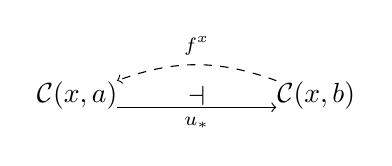
\begin{tikzpicture}[x=1.6em,y=1.2em]
  \node (xa) at (0,0) {$\mathcal{C}(x,a)$};
  \node (xb) at (5.4,0) {$\mathcal{C}(x,b)$};
  \draw[->,dashed] (4.5,0.45) to[bend right=20]
    node[above]{$\scriptstyle f^{x}$} (0.9,0.45);
  \node at (2.7,0) {$\dashv$};
  \draw[->] (0.9,-0.35) -- node[below]{$\scriptstyle u_{\ast}$} (4.5,-0.35);
\end{tikzpicture}
\end{center}
\item 对一切 $k\colon y\to x\in\mathcal{C}$，恒等 2-\trCell{}的\trMate{}是一个%
\trIsomorphism：
\begin{center}
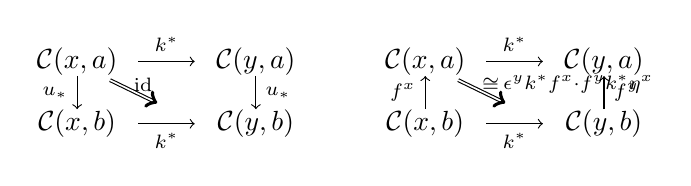
\begin{tikzpicture}[x=1.7em,y=1.5em]
  \node (xa1) at (0,1.5) {$\mathcal{C}(x,a)$};
  \node (ya1) at (3.8,1.5) {$\mathcal{C}(y,a)$};
  \node (xb1) at (0,0) {$\mathcal{C}(x,b)$};
  \node (yb1) at (3.8,0) {$\mathcal{C}(y,b)$};
  \draw[->] (1.3,1.5) -- node[above]{$\scriptstyle k^{\ast}$} (2.5,1.5);
  \draw[->] (1.3,0) -- node[below]{$\scriptstyle k^{\ast}$} (2.5,0);
  \draw[->] (0,1.15) -- node[left]{$\scriptstyle u_{\ast}$} (0,0.35);
  \draw[->] (3.8,1.15) -- node[right]{$\scriptstyle u_{\ast}$} (3.8,0.35);
  \draw[->,double] (0.7,1.05) -- (1.7,0.5);
  \node[right] at (1.0,0.95) {$\scriptstyle\mathrm{id}$};
  \node at (5.6,0.75) {$\rightsquigarrow$};
  \node (xa2) at (7.4,1.5) {$\mathcal{C}(x,a)$};
  \node (ya2) at (11.2,1.5) {$\mathcal{C}(y,a)$};
  \node (xb2) at (7.4,0) {$\mathcal{C}(x,b)$};
  \node (yb2) at (11.2,0) {$\mathcal{C}(y,b)$};
  \draw[->] (8.7,1.5) -- node[above]{$\scriptstyle k^{\ast}$} (9.9,1.5);
  \draw[->] (8.7,0) -- node[below]{$\scriptstyle k^{\ast}$} (9.9,0);
  \draw[->] (7.4,0.35) -- node[left]{$\scriptstyle f^{x}$} (7.4,1.15);
  \draw[->] (11.2,0.35) -- node[right]{$\scriptstyle f^{y}$} (11.2,1.15);
  \draw[->,double] (8.1,1.05) -- (9.1,0.5);
  \node[right] at (8.4,0.95)
    {$\scriptstyle\cong\,\epsilon^{y}k^{\ast}f^{x}\cdot f^{y}k^{\ast}\eta^{x}$};
\end{tikzpicture}
\end{center}
\end{enumerate}
\end{proposition}

\begin{proof}
\trYonedaEmbedding{} 2-\trFunctor{}
$\flat\colon\mathcal{C}\hookrightarrow\Cat^{\mathcal{C}^{\mathrm{op}}}$ 保持诸%
\trAdjunction，把 $\mathcal{C}$ 中的一个\trAdjunction{}对 $f\dashv u$ 携带为
诸可表示 2-\trFunctor{} $\mathcal{C}(-,a)$ 与 $\mathcal{C}(-,b)$ 之间的一个%
\trAdjunction
\begin{center}
\begin{tikzpicture}[x=1.7em,y=1.2em]
  \node (ma) at (0,0) {$\mathcal{C}(-,a)$};
  \node (mb) at (5.6,0) {$\mathcal{C}(-,b)$};
  \draw[->,dashed] (4.7,0.45) to[bend right=20]
    node[above]{$\scriptstyle f_{\ast}$} (1.0,0.45);
  \node at (2.8,0) {$\dashv$};
  \draw[->] (1.0,-0.35) -- node[below]{$\scriptstyle u_{\ast}$} (4.7,-0.35);
\end{tikzpicture}
\end{center}
其左与右伴随是 2-\trNaturalTransformation{} $f_{\ast}\dashv u_{\ast}$，而其%
\trUnit{}与\trCounit{}则是\trModification{}。在 $x\in\mathcal{C}$ 处求值，这便定义出如%
\cref{prop:adjunctions-representably-defined}(i)所示的一族\trAdjunction{}以及%
\textbf{严格伴随态射}（strict adjunction morphisms），意即：任何
$k\colon y\to x$ 就左、右伴随而言都诱导一个严格交换的方块，其中栖居着一对为
恒等 2-\trCell{}的\trMate{}。

真正的内容在逆命题之中。假定 (i)，定义候选的左逆
$f\coloneqq f^{b}(\mathrm{id}_{b})$。由构造
$uf\coloneqq u_{\ast}f^{b}(\mathrm{id}_{b})$，故我们可以把候选的\trUnit{}取为
$f^{b}\dashv u_{\ast}$ 的\trUnit{} $\eta^{b}$ 在 $\mathrm{id}_{b}$ 处的分量：
\[
\eta\coloneqq\mathrm{id}_{b}\;\overset{\eta^{b}_{\mathrm{id}_{b}}}{\Longrightarrow}\;uf
\qquad\in\mathcal{C}(b,b).
\]
注意到这些定义并不先验地给出关于另一复合 $fu\in\mathcal{C}(a,a)$ 的任何信息，
但条件 (ii) 定义了一个自然\trIsomorphism{} $\alpha\colon f^{a}u^{\ast}\cong u^{\ast}f^{b}$
\begin{center}
\begin{tikzpicture}[x=1.7em,y=1.5em]
  \node (sa) at (0,1.5) {$\mathcal{C}(b,a)$};
  \node (sb) at (3.8,1.5) {$\mathcal{C}(a,a)$};
  \node (sc) at (0,0) {$\mathcal{C}(b,b)$};
  \node (sd) at (3.8,0) {$\mathcal{C}(a,b)$};
  \draw[->] (1.3,1.5) -- node[above]{$\scriptstyle u^{\ast}$} (2.5,1.5);
  \draw[->] (1.3,0) -- node[below]{$\scriptstyle u^{\ast}$} (2.5,0);
  \draw[->] (0,0.35) -- node[left]{$\scriptstyle f^{b}$} (0,1.15);
  \draw[->] (3.8,0.35) -- node[right]{$\scriptstyle f^{a}$} (3.8,1.15);
  \draw[->,double] (0.7,1.05) -- (1.7,0.5);
  \node[right] at (0.95,0.95)
    {$\scriptstyle\cong\,\epsilon^{a}u^{\ast}f^{b}\cdot f^{a}u^{\ast}\eta^{b}$};
\end{tikzpicture}
\end{center}
其在 $\mathrm{id}_{b}$ 处的分量定义一个\trIsomorphism
\[
\alpha_{\mathrm{id}_{b}}\coloneqq f^{a}(u)\;
\overset{f^{a}(\eta u)}{\Longrightarrow}\;f^{a}(ufu)=f^{a}u_{\ast}(fu)\;
\overset{\epsilon^{a}(fu)}{\Longrightarrow}\;fu
\qquad\in\mathcal{C}(a,a).
\]
据此，我们把\trCounit{}定义为这个\trIsomorphism{}之逆与 $f^{a}\dashv u_{\ast}$
的\trCounit{} $\epsilon^{a}$ 在 $\mathrm{id}_{a}$ 处的分量之复合：
\[
\epsilon\coloneqq fu\;
\underset{\cong}{\overset{\alpha^{-1}_{\mathrm{id}_{b}}}{\Longrightarrow}}\;f^{a}(u)\;
\overset{\epsilon^{a}_{\mathrm{id}_{a}}}{\Longrightarrow}\;\mathrm{id}_{a}
\qquad\in\mathcal{C}(a,a).
\]
交换图
\begin{center}
\begin{tikzpicture}[x=1.6em,y=1.5em]
  \node (u)   at (0,2.6)    {$u$};
  \node (ufu) at (4.6,2.6)  {$ufu$};
  \node (ufau)   at (0,0)   {$uf^{a}(u)$};
  \node (ufaufu) at (4.6,0) {$uf^{a}(ufu)$};
  \node (ufu2) at (9.2,0)   {$ufu$};
  \draw[->,double] (0.6,2.6) -- node[above]{$\scriptstyle\eta u$} (3.9,2.6);
  \draw[->,double] (-0.4,2.1) -- node[left]{$\scriptstyle\eta^{a}(u)$} (-0.4,0.5);
  \draw[->,double] (4.6,2.1) -- node[right]{$\scriptstyle\eta^{a}(ufu)$} (4.6,0.5);
  \draw[->,double] (1.3,0) -- node[above]{$\scriptstyle u f^{a}(\eta u)$} (3.3,0);
  \draw[->,double] (6.1,0) -- node[below]{$\scriptstyle u\epsilon^{a}(fu)$} (8.0,0);
  \draw[->,double] (5.3,2.4) to[bend left=25] (9.3,0.45);
  \draw[->,double] (0.7,-0.55) to[bend right=12]
    node[below]{$\scriptstyle u\alpha_{\mathrm{id}_{b}}$} (8.6,-0.55);
\end{tikzpicture}
\end{center}
揭示出 $u\alpha_{\mathrm{id}_{b}}\cdot\eta^{a}u=\eta u$，于是
\[
u\epsilon\cdot\eta u
=(u\epsilon^{a}_{\mathrm{id}_{a}}\cdot u\alpha^{-1}_{\mathrm{id}_{b}})
 \cdot(u\alpha_{\mathrm{id}_{b}}\cdot\eta^{a}u)
=u\epsilon^{a}_{\mathrm{id}_{a}}\cdot\eta^{a}u
=\mathrm{id}_{u},
\]
这便验证了两个\trTriangleEqualities{}中的一个。%
\footnote{原书印作「$u\epsilon^{a}_{\mathrm{id}_{a}}\cdot u\alpha_{\mathrm{id}_{b}}=\mathrm{id}_{u}$」。按前一步之展开，
$u\alpha^{-1}_{\mathrm{id}_{b}}$ 与 $u\alpha_{\mathrm{id}_{b}}$ 应相消，第三段
当为 $u\epsilon^{a}_{\mathrm{id}_{a}}\cdot\eta^{a}u$（末步即由
$f^{a}\dashv u_{\ast}$ 的\trTriangleEqualities{}给出），所印
$u\alpha_{\mathrm{id}_{b}}$ 处数学不通，疑为排印之误，此处径改。——译者注}
要证明另一个\trTriangleEqualities{}的复合
\[
f\;\overset{\eta}{\Longrightarrow}\;fuf\;\overset{\epsilon}{\Longrightarrow}\;f
\qquad\in\mathcal{C}(b,a)
\]
是恒等的，则有些微妙，因为我们没有任何办法理解箭头 $f\eta$。然而注意到，这个
箭头定义了对象 $f^{b}(\mathrm{id}_{b})\in\mathcal{C}(b,a)$ 的一个自同态，于是
如果我们验证：它在\trAdjunction{} $f^{b}\dashv u_{\ast}$ 下的转置是\trUnit{}%
分量 $\eta^{b}_{\mathrm{id}_{b}}$，那么由伴随转置的唯一性，必有
$\epsilon f\cdot f\eta=\mathrm{id}_{f}$，正如所愿。这可以通过直接计算来验证：
伴随转置的计算方法是先作用\trFunctor{} $u_{\ast}$、再与
$\eta^{b}_{\mathrm{id}_{b}}=\eta$ 作预复合，这便给出下图的左下复合：
\begin{center}
\begin{tikzpicture}[x=1.6em,y=1.4em]
  \node (one) at (0,1.5)  {$1$};
  \node (uft)  at (3.6,1.5) {$uf$};
  \node (ufb)  at (0,0)   {$uf$};
  \node (ufuf) at (3.6,0) {$ufuf$};
  \node (ufbr) at (7.2,0) {$uf$};
  \draw[->,double] (0.5,1.5) -- node[above]{$\scriptstyle\eta$} (3.0,1.5);
  \draw[->,double] (-0.35,1.05) -- node[left]{$\scriptstyle\eta$} (-0.35,0.45);
  \draw[->,double] (3.6,1.05) -- node[right]{$\scriptstyle\eta uf$} (3.6,0.45);
  \draw[->,double] (0.6,0) -- node[below]{$\scriptstyle uf\eta$} (3.0,0);
  \draw[->,double] (4.3,0) -- node[below]{$\scriptstyle u\epsilon f$} (6.6,0);
  \draw[->,double] (4.2,1.4) to[bend left=25] (7.3,0.45);
\end{tikzpicture}
\end{center}
一次利用了先前验证过的\trTriangleEqualities{}的简单追图便完成了证明。
\end{proof}

\cref{prop:adjunctions-representably-defined}的条件 (ii) 被称为一个
「Beck--Chevalley」条件或\emph{正合性}条件。另一个正合性条件出现在绝对%
\trLifting{}图的一个可表示刻画之中。

\begin{definition}\label{def:right-exact-transformation}
介于如下所示的一对绝对右\trLifting{}图 $(r,\rho)$ 与 $(r',\rho')$ 之间的一个%
\trFunctor{}三元组 $(u,v,w)$ 定义一个\textbf{右正合变换}（right exact
transformation），当且仅当由绝对右\trLifting{}的\trUniversalProperty{}所诱导
的 2-\trCell{} $\tau$ 是\trInvertible：
\begin{rveq}\label{eq:right-exact-diagrams}
\mbox{\begin{tikzpicture}[x=1.55em,y=1.35em]
  \node (lb)  at (2.2,2.6)  {$b$};
  \node (lc)  at (0,1.3)    {$c$};
  \node (la)  at (2.2,1.3)  {$a$};
  \node (lbp) at (4.6,1.3)  {$b'$};
  \node (lcp) at (2.2,-1.3) {$c'$};
  \node (lap) at (4.6,-1.3) {$a'$};
  \draw[->] (0.55,1.65) -- node[above left]{$\scriptstyle r$} (1.85,2.4);
  \draw[->] (2.2,2.15) -- node[right]{$\scriptstyle f$} (2.2,1.7);
  \draw[->] (2.75,2.4) -- node[above right]{$\scriptstyle v$} (4.3,1.65);
  \node at (1.3,1.0) {$\scriptstyle\Downarrow\rho$};
  \draw[->] (0.7,1.3) -- node[below]{$\scriptstyle g$} (1.5,1.3);
  \draw[->] (0.5,0.95) -- node[below left]{$\scriptstyle w$} (1.8,-0.85);
  \draw[->] (2.65,0.95) -- node[above right]{$\scriptstyle u$} (4.15,-0.55);
  \draw[->] (4.6,0.95) -- node[right]{$\scriptstyle f'$} (4.6,-0.85);
  \draw[->] (3.0,-1.3) -- node[below]{$\scriptstyle g'$} (3.8,-1.3);
  \node at (6.0,0.65) {$=$};
  \node (rb)  at (8.2,2.6)  {$b$};
  \node (rc)  at (6.0,1.3)  {$c$};
  \node (rbp) at (10.6,1.3) {$b'$};
  \node (rcp) at (8.2,-1.3) {$c'$};
  \node (rap) at (10.6,-1.3) {$a'$};
  \draw[->] (6.55,1.65) -- node[above left]{$\scriptstyle r$} (7.85,2.4);
  \draw[->] (8.75,2.4) -- node[above right]{$\scriptstyle v$} (10.3,1.65);
  \draw[->] (6.45,0.95) -- node[below left]{$\scriptstyle w$} (7.8,-0.85);
  \draw[->] (8.6,-0.85) -- node[above left]{$\scriptstyle r'$} (10.25,1.0);
  \node at (9.0,-0.25) {$\scriptstyle\Downarrow\rho'$};
  \draw[->] (10.6,0.95) -- node[right]{$\scriptstyle f'$} (10.6,-0.85);
  \draw[->] (9.0,-1.3) -- node[below]{$\scriptstyle g'$} (9.8,-1.3);
  \node at (8.0,0.55) {$\scriptstyle\exists!\Downarrow\tau$};
\end{tikzpicture}}
\end{rveq}
\end{definition}

这个右正合性条件成立，当且仅当在 \eqref{eq:right-exact-diagrams} 左侧的图中，
经须化的 2-\trCell{} $u\rho$ 展示 $vr$ 为
$g'w$ 沿 $f'$ 的绝对右\trLifting{}——也就是说，右正合变换正是保持绝对右%
\trLifting{}图的那些变换。

\begin{lemma}\label{lem:mate-right-exact}
如下左伴随之间的交换方图
\begin{center}
\begin{tikzpicture}[x=1.8em,y=1.5em]
  \node (b)  at (1.8,1.5) {$b$};
  \node (bp) at (5.4,1.5) {$b'$};
  \node (a)  at (1.8,0)   {$a$};
  \node (ap) at (5.4,0)   {$a'$};
  \draw[->] (2.5,1.5) -- node[above]{$\scriptstyle k$} (4.7,1.5);
  \draw[->] (2.5,0) -- node[below]{$\scriptstyle h$} (4.7,0);
  \draw[->] (1.8,1.15) -- node[right]{$\scriptstyle f$} (1.8,0.35);
  \draw[->] (5.4,1.15) -- node[left]{$\scriptstyle f'$} (5.4,0.35);
  \draw[->,dashed] (1.0,0.35) to[bend left=22]
    node[left]{$\scriptstyle u$} (1.0,1.15);
  \node at (1.5,0.75) {$\scriptstyle\dashv$};
  \draw[->,dashed] (6.2,1.15) to[bend left=22]
    node[right]{$\scriptstyle u'$} (6.2,0.35);
  \node at (5.7,0.75) {$\scriptstyle\dashv$};
\end{tikzpicture}
\end{center}
的\trMate{}是\trInvertible，当且仅当 $(h,k,h)$ 定义一个介于 $\mathrm{id}_{a}$
沿 $f$ 与 $\mathrm{id}_{a'}$ 沿 $f'$ 的这两个绝对右\trLifting{}图 $(u,\epsilon)$
与 $(u',\epsilon')$ 之间的右正合变换。
\end{lemma}

\begin{proof}
满足下方\trPastingDiagram{}的那个唯一 2-\trCell{} $\tau$，即是
$\mathrm{id}\colon f'k\Rightarrow hf$ 的\trMate{}：
\begin{center}
\begin{tikzpicture}[x=1.6em,y=1.4em]
  \node (al) at (0,1.2)     {$a$};
  \node (bl) at (2.6,2.5)   {$b$};
  \node (am) at (2.6,1.2)   {$a$};
  \node (bp) at (5.8,2.5)   {$b'$};
  \node (a1l) at (3.6,-0.6) {$a'$};
  \node (a1m) at (6.4,-0.6) {$a'$};
  \draw[->] (0.4,1.4) -- node[above left]{$\scriptstyle u$} (2.2,2.3);
  \draw[->] (2.6,2.05) -- node[right]{$\scriptstyle f$} (2.6,1.6);
  \draw[double] (0.5,1.2) -- (2.1,1.2);
  \node at (1.4,1.75) {$\scriptstyle\Downarrow\epsilon$};
  \draw[->] (3.3,2.5) -- node[above]{$\scriptstyle k$} (5.1,2.5);
  \draw[->] (2.95,0.95) -- node[below left]{$\scriptstyle h$} (3.5,-0.15);
  \draw[->] (5.8,2.05) -- node[right]{$\scriptstyle f'$} (5.8,-0.1);
  \draw[double] (4.2,-0.6) -- (5.8,-0.6);
  \node at (8.3,0.9) {$=$};
  \node (ar) at (9.8,1.2)    {$a$};
  \node (br) at (12.4,2.5)   {$b$};
  \node (bpr) at (15.6,2.5)  {$b'$};
  \node (a2l) at (12.4,-0.6) {$a'$};
  \node (a2m) at (15.6,-0.6) {$a'$};
  \draw[->] (10.2,1.4) -- node[above left]{$\scriptstyle u$} (12.0,2.3);
  \draw[->] (13.1,2.5) -- node[above]{$\scriptstyle k$} (14.9,2.5);
  \draw[->] (10.2,0.95) -- node[below left]{$\scriptstyle h$} (12.1,-0.25);
  \draw[->] (12.7,-0.35) -- node[below right]{$\scriptstyle u'$} (15.0,2.15);
  \draw[->] (15.6,2.05) -- node[right]{$\scriptstyle f'$} (15.6,-0.1);
  \draw[double] (13.0,-0.6) -- (15.0,-0.6);
  \node at (13.3,1.15) {$\scriptstyle\exists!\Downarrow\tau$};
  \node at (14.95,0.5) {$\scriptstyle\Downarrow\epsilon'$};
\end{tikzpicture}
\end{center}
\end{proof}

\begin{proposition}\label{prop:absolute-right-lifting-representable}
考虑一个 2-\trCategory{} $\mathcal{C}$ 中的 2-\trCell{}
\begin{center}
\begin{tikzpicture}[x=1.6em,y=1.4em]
  \node (b) at (2.6,2.2) {$b$};
  \node (c) at (0,0) {$c$};
  \node (a) at (2.6,0) {$a$};
  \draw[->] (0.5,0.35) -- node[above left]{$\scriptstyle r$} (2.2,1.95);
  \draw[->] (2.6,1.75) -- node[right]{$\scriptstyle f$} (2.6,0.45);
  \node at (1.6,0.75) {$\scriptstyle\Downarrow\rho$};
  \draw[->] (0.6,0) -- node[below]{$\scriptstyle g$} (2.0,0);
\end{tikzpicture}
\end{center}
\begin{enumerate}[label=(\roman*)]
\item 若 $(r,\rho)$ 在 $\mathcal{C}$ 中定义一个绝对右\trLifting{}图，则
  \begin{enumerate}[label=(\alph*)]
  \item 对一切 $x\in\mathcal{C}$，
\begin{center}
\begin{tikzpicture}[x=1.6em,y=1.4em]
  \node (xb) at (2.6,2.2) {$\mathcal{C}(x,b)$};
  \node (xc) at (0,0) {$\mathcal{C}(x,c)$};
  \node (xa) at (2.6,0) {$\mathcal{C}(x,a)$};
  \draw[->] (0.5,0.35) -- node[above left]{$\scriptstyle r_{\ast}$} (2.2,1.95);
  \draw[->] (2.6,1.75) -- node[right]{$\scriptstyle f_{\ast}$} (2.6,0.45);
  \node at (1.7,0.75) {$\scriptstyle\Downarrow\rho_{\ast}$};
  \draw[->] (0.7,0) -- node[below]{$\scriptstyle g_{\ast}$} (2.0,0);
\end{tikzpicture}
\end{center}
    在 $\Cat$ 中定义一个绝对右\trLifting{}图。
  \item 对一切 $k\colon w\to x\in\mathcal{C}$，所诱导的变换是右正合的。
\begin{center}
\begin{tikzpicture}[x=1.9em,y=1.4em]
  \node (xcb) at (3.4,2.6) {$\mathcal{C}(x,b)$};
  \node (xcc) at (0,1.3) {$\mathcal{C}(x,c)$};
  \node (xca) at (3.4,1.3) {$\mathcal{C}(x,a)$};
  \node (cwb) at (6.8,1.3) {$\mathcal{C}(w,b)$};
  \node (cwc) at (3.4,-1.3) {$\mathcal{C}(w,c)$};
  \node (cwa) at (6.8,-1.3) {$\mathcal{C}(w,a)$};
  \draw[->] (3.4,2.2) -- node[right]{$\scriptstyle f_{\ast}$} (3.4,1.75);
  \draw[->] (4.3,2.4) -- node[above right]{$\scriptstyle k^{\ast}$} (6.1,1.6);
  \draw[->] (1.0,1.3) -- node[below]{$\scriptstyle g_{\ast}$} (2.2,1.3);
  \draw[->] (0.8,0.95) -- node[below left]{$\scriptstyle k^{\ast}$} (2.7,-0.85);
  \draw[->] (4.3,0.95) -- node[above left]{$\scriptstyle k^{\ast}$} (6.2,-0.9);
  \draw[->] (6.8,0.95) -- node[right]{$\scriptstyle f_{\ast}$} (6.8,-0.85);
  \draw[->] (4.4,-1.3) -- node[below]{$\scriptstyle g_{\ast}$} (5.6,-1.3);
\end{tikzpicture}
\end{center}
  \end{enumerate}
\item 反之，若 ((a)) 对每个 $x\in\mathcal{C}$ 都成立，则 $(r,\rho)$ 在
  $\mathcal{C}$ 中定义一个绝对右\trLifting{}图。
\item 此外，若 $g\colon c\to a$ 与 $f\colon b\to a$ 使得对一切
  $x\in\mathcal{C}$，\trFunctor{} $g_{\ast}\colon\mathcal{C}(x,c)\to\mathcal{C}(x,a)$
  容许一个沿 $f_{\ast}\colon\mathcal{C}(x,b)\to\mathcal{C}(x,a)$ 的绝对右%
  \trLifting{}且条件 ((b)) 对其成立，则 $g$ 在 $\mathcal{C}$ 中容许一个沿 $f$
  的绝对右\trLifting。
\end{enumerate}
\end{proposition}

\begin{proof}
第一个陈述最为直接，我们将其证明留给读者，提示是：为验证 $\Cat$ 中一个绝对%
\trLifting{}图的\trUniversalProperty，只需考虑余跨度 $(g_{\ast},f_{\ast})$
之上以终\trCategory{} $1$ 为顶点的那些\trCone。

对于第二个断言，考虑 $\mathcal{C}$ 中余跨度 $(g,f)$ 之上的一个\trCone
\begin{center}
\begin{tikzpicture}[x=1.6em,y=1.4em]
  \node (x) at (0,1.7) {$x$};
  \node (b) at (3.0,1.7) {$b$};
  \node (c) at (0,0) {$c$};
  \node (a) at (3.0,0) {$a$};
  \draw[->] (0.5,1.7) -- node[above]{$\scriptstyle y$} (2.5,1.7);
  \draw[->] (0,1.25) -- node[left]{$\scriptstyle z$} (0,0.45);
  \draw[->] (3.0,1.25) -- node[right]{$\scriptstyle f$} (3.0,0.45);
  \draw[->] (0.6,0) -- node[below]{$\scriptstyle g$} (2.4,0);
  \node at (1.5,0.85) {$\scriptstyle\Downarrow\chi$};
\end{tikzpicture}
\end{center}
这份数据定义了如下图左侧所示的一个\trCategory{}图表，它唯一地分解成右侧所示的
形状：
\begin{center}
\begin{tikzpicture}[x=1.6em,y=1.4em]
  \node (one) at (0,1.7) {$1$};
  \node (cxb) at (3.6,1.7) {$\mathcal{C}(x,b)$};
  \node (cxc) at (0,0) {$\mathcal{C}(x,c)$};
  \node (cxa) at (3.6,0) {$\mathcal{C}(x,a)$};
  \draw[->] (0.4,1.7) -- node[above]{$\scriptstyle y$} (2.4,1.7);
  \draw[->] (0,1.25) -- node[left]{$\scriptstyle z$} (0,0.45);
  \draw[->] (3.6,1.25) -- node[right]{$\scriptstyle f_{\ast}$} (3.6,0.45);
  \draw[->] (0.8,0) -- node[below]{$\scriptstyle g_{\ast}$} (2.4,0);
  \node at (1.5,0.85) {$\scriptstyle\Downarrow\chi$};
  \node at (5.2,0.85) {$=$};
  \node (one2) at (6.8,1.7) {$1$};
  \node (cxb2) at (10.6,1.7) {$\mathcal{C}(x,b)$};
  \node (cxc2) at (6.8,0) {$\mathcal{C}(x,c)$};
  \node (cxa2) at (10.6,0) {$\mathcal{C}(x,a)$};
  \draw[->] (7.2,1.7) -- node[above]{$\scriptstyle y$} (9.4,1.7);
  \draw[->] (6.8,1.25) -- node[left]{$\scriptstyle z$} (6.8,0.45);
  \draw[->] (10.6,1.25) -- node[right]{$\scriptstyle f_{\ast}$} (10.6,0.45);
  \draw[->] (7.6,0) -- node[below]{$\scriptstyle g_{\ast}$} (9.4,0);
  \node at (8.7,1.0) {$\scriptstyle\exists!\Downarrow\zeta$};
  \draw[->,dashed] (8.2,0.35) -- node[below left]{$\scriptstyle r_{\ast}$} (10.0,1.45);
  \node at (9.7,0.6) {$\scriptstyle\Downarrow\rho_{\ast}$};
\end{tikzpicture}
\end{center}
从而定义出所求的唯一分解
\begin{center}
\begin{tikzpicture}[x=1.6em,y=1.4em]
  \node (x) at (0,1.7) {$x$};
  \node (b) at (3.0,1.7) {$b$};
  \node (c) at (0,0) {$c$};
  \node (a) at (3.0,0) {$a$};
  \draw[->] (0.5,1.7) -- node[above]{$\scriptstyle y$} (2.5,1.7);
  \draw[->] (0,1.25) -- node[left]{$\scriptstyle z$} (0,0.45);
  \draw[->] (3.0,1.25) -- node[right]{$\scriptstyle f$} (3.0,0.45);
  \draw[->] (0.6,0) -- node[below]{$\scriptstyle g$} (2.4,0);
  \node at (1.5,0.85) {$\scriptstyle\Downarrow\chi$};
  \node at (4.4,0.85) {$=$};
  \node (x2) at (5.8,1.7) {$x$};
  \node (b2) at (8.8,1.7) {$b$};
  \node (c2) at (5.8,0) {$c$};
  \node (a2) at (8.8,0) {$a$};
  \draw[->] (6.3,1.7) -- node[above]{$\scriptstyle y$} (8.3,1.7);
  \draw[->] (5.8,1.25) -- node[left]{$\scriptstyle z$} (5.8,0.45);
  \draw[->] (8.8,1.25) -- node[right]{$\scriptstyle f$} (8.8,0.45);
  \draw[->] (6.4,0) -- node[below]{$\scriptstyle g$} (8.2,0);
  \node at (7.2,0.95) {$\scriptstyle\Downarrow\zeta$};
  \draw[->,dashed] (6.4,0.35) -- node[below left]{$\scriptstyle r$} (8.2,1.45);
  \node at (8.0,0.55) {$\scriptstyle\Downarrow\rho$};
\end{tikzpicture}
\end{center}
对于最后一个断言，我们把 $(r,\rho)$ 定义为：将所假定的绝对右\trLifting{}
$(r^{c},\rho^{c})$ 的那个\trFunctor{}与那个\trNaturalTransformation{}在情形
$x=c$ 之下于 $\mathrm{id}_{c}\in\mathcal{C}(c,c)$ 处求值。为验证
$\rho\colon fr\Rightarrow g$ 定义 $g$ 沿 $f$ 的一个绝对右\trLifting，考虑一支
1-\trCell{} $z\colon x\to c$。右正合性假设告诉我们，复合变换
\begin{center}
\begin{tikzpicture}[x=1.9em,y=1.4em]
  \node (ccb) at (5.0,2.6) {$\mathcal{C}(c,b)$};
  \node (one) at (0,1.3) {$1$};
  \node (ccc) at (2.6,1.3) {$\mathcal{C}(c,c)$};
  \node (cca) at (5.0,1.3) {$\mathcal{C}(c,a)$};
  \node (cxb) at (8.8,1.4) {$\mathcal{C}(x,b)$};
  \node (cxc) at (5.2,-1.3) {$\mathcal{C}(x,c)$};
  \node (cxa) at (8.8,-1.3) {$\mathcal{C}(x,a)$};
  \draw[->] (0.45,1.3) -- node[above]{$\scriptstyle\mathrm{id}_{c}$} (1.65,1.3);
  \draw[->,dashed] (3.2,1.65) -- node[above left]{$\scriptstyle r^{c}$} (4.6,2.4);
  \node at (3.9,0.95) {$\scriptstyle\Downarrow\rho^{c}$};
  \draw[->] (5.05,2.2) -- node[left]{$\scriptstyle f_{\ast}$} (5.0,1.75);
  \draw[->] (5.9,2.4) -- node[above right]{$\scriptstyle z^{\ast}$} (8.2,1.65);
  \draw[->] (3.4,1.3) -- node[below]{$\scriptstyle g_{\ast}$} (4.15,1.3);
  \draw[->] (8.8,1.0) -- node[right]{$\scriptstyle f_{\ast}$} (8.8,-0.85);
  \draw[->] (3.2,0.95) -- node[below left]{$\scriptstyle z^{\ast}$} (4.9,-0.85);
  \draw[->] (5.7,0.95) -- node[above left]{$\scriptstyle z^{\ast}$} (8.2,-0.95);
  \draw[->] (6.1,-1.3) -- node[below]{$\scriptstyle g_{\ast}$} (7.9,-1.3);
\end{tikzpicture}
\end{center}
是绝对右\trLifting。由上文第二个断言的证明，这告诉我们 $(r^{c},\rho^{c})$ 是
$g_{\ast}$ 沿 $f_{\ast}$ 的一个绝对右\trLifting，从而证得 $(r,\rho)$ 如所求地
是一个绝对右\trLifting。
\end{proof}

\begin{remark}\label{rem:yoneda-perspective}
\cref{prop:adjunctions-representably-defined}与
\cref{prop:absolute-right-lifting-representable}的结果可视为\trBicategorical{} Yoneda
引理的一些应用，后者定义了从\trBicategory{} $\mathcal{C}$ 到由伪函子、伪自然变换与%
\trModification{}组成的 2-\trCategory{} $[\mathcal{C}^{\mathrm{op}},\Cat]$ 的一个%
2-\trFullyFaithful{}嵌入（见第 10 章中的\cref{def:pseudofunctor}、第 10 章中
的\cref{def:pseudonatural-transformation}与附录 B 中的\cref{def:modification}）。
若 $\mathcal{C}$ 中的一支 1-\trCell{} $u\colon a\to b$ 满足%
\cref{prop:adjunctions-representably-defined}的条件 (i)，则由附录 B 中的%
\cref{thm:mates-double-functoriality}，诸\trLeftAdjoint{}
$f^{x}\colon\mathcal{C}(x,b)\to\mathcal{C}(x,a)$ 定义一个%
\trOplax\trNaturalTransformation{}的诸分量。条件 (ii) 要求这个%
\trOplax\trNaturalTransformation{}是一个伪自然变换。如今，2-全忠实性使我们
能把这一点提升为 $\mathcal{C}$ 中的一支箭头 $f\colon b\to a$，后者是 $u$ 的%
\trLeftAdjoint。

至于\cref{prop:equivalences-representably-defined}的情形——其中
$u\colon a\to b$ 诱导诸\trEquivalence{}
$\mathcal{C}(x,a)\Rightarrow\mathcal{C}(x,b)$——诸逆可以经选取而定义%
\trAdjointEquivalence，后者自动地拼装成一个伪自然变换（见第 10 章中的%
\cref{lem:adjoint-inverses-qpn}）。这正是无需任何附加假设的原因。
\end{remark}

\subsection*{练习}

\begin{exercise}\label{ex:confirm-mate-assertion}
确证\cref{lem:mate-right-exact}的证明中所述的论断。
\end{exercise}

\begin{exercise}\label{ex:prove-representable-absolute-lifting}
证明\cref{prop:absolute-right-lifting-representable}(i)。
\end{exercise}

   %
